% This is a latex file for Journal Club report 


% Author: Viswambhar Yasa
\documentclass[a4paper,12pt,times]{article}

% This are some packages used in bulding the report 
\usepackage{amsmath} 
\usepackage{graphicx}
\usepackage{multirow}
\usepackage{fancyvrb,color}
\usepackage{float}
\usepackage{amsmath}
\usepackage{geometry}
\usepackage[sort&compress,square,comma,numbers]{natbib}
\usepackage{wrapfig, blindtext}
\usepackage{index}
\usepackage[intoc]{nomencl}
\usepackage{subfig}
\usepackage{matlab-prettifier}
\usepackage{csvsimple}
\usepackage[english]{babel}
\usepackage{hyperref}
\hypersetup{
    colorlinks=true,
    linkcolor=blue,
    filecolor=blue,      
    urlcolor=blue,
}
\usepackage{listings}
\usepackage{color}

\definecolor{dkgreen}{rgb}{0,0.6,0}
\definecolor{gray}{rgb}{0.5,0.5,0.5}
\definecolor{mauve}{rgb}{0.58,0,0.82}

\lstset{frame=tb,
  language=Python,
  aboveskip=3mm,
  belowskip=3mm,
  showstringspaces=false,
  columns=flexible,
  basicstyle={\small\ttfamily},
  numbers=none,
  numberstyle=\tiny\color{gray},
  keywordstyle=\color{blue},
  commentstyle=\color{dkgreen},
  stringstyle=\color{mauve},
  breaklines=true,
  breakatwhitespace=true,
  tabsize=3
}


\setlength{\parindent}{1em}
\setlength{\parskip}{0.5em}
\renewcommand{\baselinestretch}{1}

\def\myauthor{Viswambhar Reddy Yasa} % Author
\def\matriculationno{65074} 
\def\mytitle{iso-geometric analysis based topology optimization (igto) }
\def\mydate{\today} 

%start  of the main documnt
\begin{document}

%This is calling out sub-latex file in our main latex file

\begin{titlepage}

    \begin{center}
    \textsc{Personal Programming Project 2020-21 }\\
    \vspace*{0.5 cm}
    {\LARGE \textsc{\mytitle}} %Title 
    \vspace{0.025\textheight}
    \rule{0.75\textwidth}{0.45pt}\\
    \vspace*{1 cm}
    
    \includegraphics[scale=0.6]{WBM_schwarz.png}\\
    \vspace*{2.5 cm}
    {\large \textsc{\myauthor}}\\ % Name
    \vspace{0.025\textheight}
    {\textsc{Computational Material Science}}\\
	\vspace{0.025\textheight}
	{65074}\\
	\vspace{2 cm}
	\textsc{Supervised by}\\
	\vspace{0.0025\textheight}
	{\textsc{Dr.-Ing. Martin Abendroth}}\\
	\vfill
	\textsc{Professor Incharge}\\
	\vspace{0.0025\textheight}
	{\textsc{Dr.-Ing Arun Prakash and Dr.-Ing Habil Geralf Hutter}}\\
	\vspace{2 cm}
	{\mydate}
    \vspace{0.25\textheight}     	
	\rule{\textwidth}{1.5pt} 
    \end{center} 
         
\end{titlepage}

\tableofcontents
\vfill
%\pagebreak to move to next page
\numberwithin{equation}{section}
%this is the introduction section
\newpage
\begin{section}{Introduction}
Iso-Geometric Analysis(IGA) is a recently developed method in which the Computer Aided Design (CAD) is integrated with Computer Aided Engineering (CAE). In Computer Aided Engineering, we utilize finite element method to find approximate solution of the problem.This approximation is done by discretizing the geometry into smaller parts known as elements.

In many standard design tools, basis splines (B splines) are the basis used to create elements like curves, lines and surfaces. Standard Finite element method uses Lagrangian function as their basics, what-if we use B splines or NURBS(Non-Uniform Rational B-Splines) as basics function for FEM which lead to the formulation of ISO-geometric analysis. In ISO-geometric analysis, there is a tight coupling between design(CAD) and analysis (CAE) such that the geometry is captured exactly eliminating any error due to geometric approximation. 

\begin{subsection}{Advantages of IGA over standard FEM}
\begin{itemize}
\item Smooth contact surface can be obtained without geometrical approximation, leading to more physically accurate contact stresses.$^{\cite{NGUYEN201589}}$
  \item Due to integrating of CAE and CAD, we save a lot time but eliminating geometric discretization.
  
  \item IGA has been applied to cohesive fracture, outlining a framework for modeling debonding along material
interfaces using NURBS.$^{\cite{NGUYEN201589}}$
  
  \item Due to strong coupling with geometry, optimization problem can be solved effectively. This lead us to use IGA for structural topology optimization.
  
\end{itemize}
\end{subsection}

\begin{subsection}{Topology optimization using IGA}
The main idea behind structural optimization is to get structures with minimum weight for different stresses and design constraints. Topology optimization is a mathematical method of optimizing the distribution of material within the domain so that the structure would satisfy the design parameters. The design parameters include geometry of the domain, applied load and position of the load, the amount of mass which has remain after optimization. We implemented SIMP(Solid Isotropic Material with Penalization) method in order to remove porosity as this method is quite effective for minimum weight topology. 
$^{\cite{Okruta2014ThreedimensionalTO}}$ 
\end{subsection}

The main objective of personal programming project is to develop a python code which could implement topology optimization of a structure using a mesh-less method(IGA). First, the structure is analysed using IGA and compliance is calculated. Based on the compliance and volume constrains, we used optimality criterion and Method of moving asymptotes to solve constrained based non-linear optimization problem. The optimization of structure is performed until the termination criteria is satisfied.

\end{section}

\begin{section}{Basis Splines}
In CAD to represent geometrical objects we require different type of discretisation which cannot be achieved using Bezier curves or Lagrange polynominal. So basis splines based method NURBS are used to get desired properties for interactive geometrical design.$^{\cite{NGUYEN201589}}$. Fig[\ref{fig:Cubic B-Spline}] shows a Cubic B-spline.

To construct a B-spline , the control points and degree of the curve have to be specified. Based on which the knot vector is developed.$^{\cite{NGUYEN201589}}$. 


\begin{figure}[h!]
\centering
\includegraphics[width=0.75\linewidth]{Bsplines_figure1.png}
\caption{Cubic B-spline with 6 control points.$^{\cite{lockyer2007controlling}}$}
\label{fig:Cubic B-Spline}
\end{figure}

\begin{subsection}{Control points}
In FEM, we need nodes to generate mesh similarly in IGA we require control points which are co-ordinates of the curve. The shape of the curve depends on the control point position and degree of the B-spline. Control points for complex geometries can be download as text file from any design software. 
\end{subsection}

\begin{subsection}{Degree of the B-spline}
The order or degree of B-splines represents the number of control point which influence the position of the curve. This can be clearly seen in  Fig[\ref{fig:B-spline for various degrees}]. The maximum degree of the B-spline curve is one less then the number of control points.

\begin{figure}[h!]
\centering
\includegraphics[width=0.9\linewidth]{Bspline_curve_different_order.png}
\caption{B-spline with 9 control points plotted for different degrees.}
\label{fig:B-spline for various degrees}
\end{figure}

\end{subsection}

\begin{subsection}{Generation of Knot vector}
The spacing of knots in the knot vector has a significant effect on the shape of a B-spline curve. In IGA, knot vector is an array of values arranged in ascending order. A knot vector divides the knot span into elements known as patches.


Knot vector ${\displaystyle \xi =\{\xi _{1},\xi _{2},...,\xi _{n+p+1}\}}$,${\displaystyle n}$ is the number of functions, ${\displaystyle p}$ refers to the basis functions degree.

The simplest method of specifying knot vector is by evenly spacing. If the first and the last knots appear ${\displaystyle p+1}$ times, the knot vector is said to be open else clamped .As shown in Fig[\ref{fig:B-spline curve of evenly space open clamped knot vector}].\\


\begin{figure}[h!]
\centering
\includegraphics[width=0.75\linewidth]{knot_vector_clamped_unclamped.png}
\caption{B-spline curve of open and clamped knot vector.$^{\cite{lockyer2007controlling}}$}
\label{fig:B-spline curve of evenly space open clamped knot vector}
\end{figure}

\begin{lstlisting}
    def knot_vector(self, n, degree):
        '''
        This function return knotvector based on the number of control points and degree of Bspline
        Parameters
        ----------
        control_points : int
            number of points along with weights.
        degree : int
            order of B-splines  0-constant, 1-linear, 2-quadratic, 3-cubic.

        Returns
        -------
        KNOTVECTOR - an array containing knots based on control points

        Test case
        ------
        test command - 
                        pytest test_Inputs.py::test__knotvector_true
        '''
\end{lstlisting}

The function knot vector is implemented as method in Input class.
To run the test case. 

\begin{lstlisting}
(1) pytest test_Inputs.py::test__knotvector_true
\end{lstlisting}
The function output is compared with the value obtained from NURBS book $^{\cite{10.5555/265261}}$.


\begin{figure}[h!]
\centering
\includegraphics[width=\linewidth]{knot_vector_combined.png}
\caption{Knot vector and B-spline curve change due to change in degree.}
\label{fig:change in knot vector and B-spline curve due to change in degree}
\end{figure}

\end{subsection}
\begin{subsection}{B-spline Basis function}
B-spline basis function is defined using recursive formula i.e Cox-de-Boor formulation, starting with the zeroth order basis function (p = 0).$^{\cite{NGUYEN201589}}$. 


\begin{equation}\label{Cox-de-Boor formula zero basics}
N_{i, 0}(\xi)=\left\{\begin{array}{ll}
1 & \text { if } \xi_{i} \leq \xi<\xi_{i+1} \\
0 & \text { otherwise }
\end{array}\right.
\end{equation}

and for a polynomial order p greater then one
\begin{equation}\label{Cox-de-Boor formula higher order}
N_{i, p}(\xi)=\frac{\xi-\xi_{i}}{\xi_{i+p}-\xi_{i}} N_{i, p-1}(\xi)+\frac{\xi_{i+p+1}-\xi}{\xi_{i+p+1}-\xi_{i+1}} N_{i+1, p-1}(\xi) .
\end{equation}

\begin{figure}[h!]
\centering
\includegraphics[width=0.75\linewidth]{Bspline_basis_recussive.png}
\caption{B-spline basis dependancy on other basis.$^{\cite{owens2009implementation}}$}
\label{fig:B-spline basis dependancy on other basis}
\end{figure}


B-splines function are not interpolatory i.e, value does not pass through them but the curves are approximated based on the values . Fig[\ref{fig:B-spline basis dependancy on other basis}] show how the higher order basis functions depend on lower order basis functions.

 
\begin{lstlisting} 

def bspline_basis(knot_index,degree,U,knotvector):
    '''
    modified version based on Algorthim 2.2 THE NURBS book pg70
    Implementation of equation 2.2 for the documentation

    Generates Basis functions.
    Parameters
    ----------
    knotindex : int 
        DESCRIPTION. The default is ''.
    degree : int
        order of B-splines  0-constant, 1-linear, 2-quadratic, 3-cubic
    U : int
            The value whose basis are to be found
    knotvector : array or list
            list of knot values.
    Returns
    -------
    Basis: Array dimension degree+1   
            It contains non-zero cox de boor based basis function
                Ex= if degree=2 and knotindex=4 
                    basis=[N 2_0, N 3_1, N 4_2]
    '''
\end{lstlisting}
\subsubsection{Properties of B-spline basis function}
%\begin{subsubsection}{Properties of B-spline basis function}

Some properties of B-spline basis function. The values for the test cases are obtained from the NURBS book.$^{\cite{10.5555/265261}}$.
\begin{itemize}
\item They constitute a partition of unity.


\item Each basis function is non-negative over the entire parametric domain

\item They are linearly independent
\end{itemize}
Given below are respective commands to run the test cases
\begin{lstlisting} 

(2) pytest test_geometry.py::test__Bspline_basis_sum_equal_to_one_true

(3) pytest test_geometry.py::test__Bspline_basis_all_values_positive_true

(4) pytest test_geometry.py::test__Bspline_basis_equal_true
\end{lstlisting}

\subsubsection{Derivatives of B-spline functions}
To implement FEM, we require the derivatives of the basis function. For IGA the first order derivatives are sufficient.

\begin{equation}\label{B-spline Derivative}
\frac{d}{d \xi} N_{i, p}(\xi)=\frac{p}{\xi_{i+p}-\xi_{i}} N_{i, p-1}(\xi)-\frac{p}{\xi_{i+p+1}-\xi_{i+1}} N_{i+1, p-1}(\xi)
\end{equation}  
\begin{lstlisting}

def derbspline_basis(knot_index,degree,U,knotvector,order=1):
    """
    Modified version based on the alogorithm A2.3 
    in NURBS Book page no.72
    Parameters
    ----------
    knot_index : integer
                The position of the value U in knotvector
    degree : int
        order of B-splines  0-constant, 1-linear, 2-quadratic,
         3-cubic
    U : int
            The value whose basis are to be found
    knotvector : array or list
            list of knot values.
            
	order :int 
		default :1
		
    Returns
    -------
    Array 
        Derivatives of Basis array of dimension degree+1
        It contains non-zero cox de boor based basis function
            Ex= if degree=2 and knotindex=4 
            der_basis=[N' 2_0, N' 3_1, N' 4_2].
      """

\end{lstlisting}

\begin{figure}[h!]
\centering
\includegraphics[width=0.75\linewidth]{bspline_function_and_derivative_cubic.png}
\caption{a)Cubic B-spline basis function b) Cubic B-spline derivative function .$^{\cite{10.5555/265261}}$}
\label{fig:Cubic Bspline basis function and it's derivative}
\end{figure}

\paragraph{Properties of B-spline basis function derivatives}
%\begin{subsubsection}{Properties of B-spline basis function}
Some properties of derivatives of B-spline basis function. The values for the test cases are obtained from the NURBS book.$^{\cite{10.5555/265261}}$.
 
\begin{itemize}
\item Derivative of basis functions sum upto to zero $\sum_{i=0}^{n}d N_{i, p}(\xi)=0$.

\item They are linearly independent

\end{itemize}
Given below are respective commands to run the test cases.
\begin{lstlisting} 

(5) pytest test_geometry.py::test__derbspline_basis_sum_equal_zero_true

(6) pytest test_geometry.py::test__derbspline_basis_equal_true

\end{lstlisting}
%\end{subsection}
\end{subsection}


\end{section}


\begin{section}{NURBS (Non-Uniform Rational B-splines) }
B-spline are useful for free-form drawing but lack the flexibility to represent simple geometry like circle and ellipsoid. Therefore NURBS are used which make use of weight functions and have the ability to form exact representation of circles, paraboloids and ellipsoids.

In Fig[\ref{fig:NURBS and B-splines representation and differance}] NURBS with weight equal to one represent B-splines. 

\begin{figure}[h!]
\centering
\includegraphics[width=\linewidth]{NURBS_combined_bspline.png}
\caption{a) B-spline b) NURBS}
\label{fig:NURBS and B-splines representation and differance}
\end{figure}

\begin{subsection}{NURBS basis function}
Similar to B-spline basis function, NURBS depend on additional weight parameter.
It is defined as:
\begin{equation}\label{NURBS basis function}
R_{i, p}(\xi)=\frac{N_{i, p}(\xi) w_{i}}{W(\xi)}=\frac{N_{i, p}(\xi) w_{i}}{\sum_{i=1}^{n} N_{\hat{i}, p}(\xi) w_{i}}
\end{equation}

By selecting appropriate weights, we can describe many type of curves.  

\begin{figure}[h!]
\centering
\includegraphics[width=0.85\linewidth]{NURBS_circle.png}
\caption{Circle from NURBS}
\label{fig:NURBS circle for different degree}
\end{figure}

NURBS has to satisfy all properties of B-splines, NURBS are function of B-splines and form superset of them.

\end{subsection}

\begin{subsection}{NURBS derivative function}
The first derivative of a NURBS basis function is computed using the quotient rule as $^{\cite{owens2009implementation}}$

\begin{equation}\label{NURBS derivatives}
\frac{d}{d \xi} R_{i, p}(\xi)=w_{i} \frac{N_{i, p}^{\prime}(\xi) W(\xi)-N_{i, p}(\xi) W^{\prime}(\xi)}{W(\xi)^{2}}
\end{equation}

$\text { where } N_{i, p}^{\prime}(\xi) \equiv \frac{d}{d \xi} N_{i, p}(\xi) \text { and }$
\begin{equation}\label{weights}
W^{\prime}(\xi)=\sum_{\hat{i}=1}^{n} N_{i, p}^{\prime}(\xi) w_{i}^{n}
\end{equation}
\end{subsection}

\begin{subsection}{NURBS volume}
The most important relation required for IGA is the NURBS volume which is the tensor product of NURBS basis in 3 directions.
\begin{equation}\label{NURBS volume}
V(\xi, \eta, \zeta)=\sum_{i=0}^{n} \sum_{j=0}^{m} \sum_{k=0}^{l} R_{i, j, k}^{p, q, r}(\xi, \eta, \zeta) P_{i, j, k}
\end{equation}

\begin{figure}[h!]
\centering
\includegraphics[width=0.75\linewidth]{NURBS_2D_surface.png}
\caption{ NURBS surface.$^{\cite{owens2009implementation}}$}
\label{fig:NURBS surface}
\end{figure}

where the trivariant function is given as
\begin{equation}\label{Trivariant function}
R_{i, j, k}^{p, q, r}(\xi, \eta, \zeta)=\frac{N_{i, p}(\xi) N_{j, q}(\eta) N_{k, r}(\zeta) w_{i, j, k}}{\sum_{i=0}^{n} \sum_{j=0}^{m} \sum_{k=0}^{l} N_{i, p}(\xi) N_{j, q}(\eta) N_{k, r}(\zeta) w_{i, j, k}}
\end{equation}

For easy representation,As shown in fig[\ref{fig:NURBS surface}] a surface is considered. In 2D, Control points form a net and knot vector along t1,t2 form patches. In 3D, knot vector along U,V,W form a patches.

\subsubsection{Derivative of Trivariant basis function}
Derivative of trivariant basis function follow chain rule
\begin{equation}
\frac{\partial R_{i, j,k}^{p, q,r}}{\partial \xi}=\frac{N_{i, p}^{\prime} N_{j, q}N_{k, r} W-N_{i, p} N_{j, q} N_{k, r}W_{\xi}^{\prime}}{W^{2}} w_{i, j}
\end{equation}

\begin{equation}
\frac{\partial R_{i, j,k}^{p, q,r}}{\partial \eta}=\frac{N_{i, p} N_{j, q}^{\prime}N_{k, r} W-N_{i, p} N_{j, q} N_{k, r}W_{\eta}^{\prime}}{W^{2}} w_{i, j}
\end{equation}


\begin{equation}
\frac{\partial R_{i, j,k}^{p, q,r}}{\partial \zeta}=\frac{N_{i, p} N_{j, q}N_{k, r}^{\prime} W-N_{i, p} N_{j, q} N_{k, r}W_{\zeta}^{\prime}}{W^{2}} w_{i, j}
\end{equation}
where
\begin{equation}
W=\sum_{i=0}^{n} \sum_{j=0}^{m}\sum_{k=0}^{l} N_{i, p} N_{j, q} N_{k, r}w_{i, j}
\end{equation}

\begin{equation}
W_{\xi}^{\prime}=\sum_{i=0}^{n} \sum_{j=0}^{m} \sum_{k=0}^{k} N_{i, p}^{\prime} N_{j, q} N_{k, r} w_{i, j}
\end{equation}

\begin{equation}
W_{\eta}^{\prime}=\sum_{i=0}^{n} \sum_{j=0}^{m} \sum_{k=0}^{k} N_{i, p} N_{j, q}^{\prime} N_{k, r} w_{i, j}
\end{equation}

\begin{equation}
W_{\zeta}^{\prime}=\sum_{i=0}^{n} \sum_{j=0}^{m} \sum_{k=0}^{k} N_{i, p} N_{j, q} N_{k, r}^{\prime} w_{i, j}
\end{equation}
\end{subsection}
\begin{lstlisting}
def trilinear_der(Ux,Uy,Uz,weights,xdegree,xknotvector,ydegree,yknotvector,
zdegree,zknotvector):
    '''
    NURBS volume which is a tensor product of NURBS basis along xi,eta,neta direction.
    Parameters
    ----------
    Ux,Uy,Uz : float
                knot index along xi,eta,neta direction
    weights : Array 
                An array of NURBS weights defined for each knot.
    xdegree,ydegree,zdegree : int
                   degree of the knotvector along xi,eta,neta
                   0-constant, 1-linear, 2-quadratic, 3-cubic
    xknotvector,yknotvector,zknotvector : Array
                     knotvectors defined along xi,eta,neta
    Returns
    -------
    R - Array.
        Trivariant function 
    dR_dx,dR_dy,dR_dz -Array
        Derivative of Trivariant function along xi,eta,neta direction.
    '''
\end{lstlisting}
The values for the test cases are obtained from the NURBS book$^{\cite{10.5555/265261}}$.Given below are respective commands to run the test cases
\begin{lstlisting}

(7) pytest test_geometry.py::test__trilinear_der_Basis_sum_equal_to_one_true

(8) pytest test_geometry.py::test__trilinear_der_Basis_less_than_zero_false

(9) pytest test_geometry.py::test__trilinear_der_XI_sum_equal_to_zero_true

(10) pytest test_geometry.py::test__trilinear_der_ETA_sum_equal_to_zero_true

(11) pytest test_geometry.py::test__trilinear_der_NETA_sum_equal_to_zero_true

\end{lstlisting}
\end{section}

%%%%%%%%%%%%%%%%
\begin{section}{Background Theory}
\begin{subsection}{Constitutive equation and their weak form}
Based on conservation of linear momentum. The equilibrium equation is given below.
\begin{equation}\label{strong form}
\sigma_{i j, j}+f_{i}=0
\end{equation}
The $\sigma_{i j, j}$ is known as stress tensor and f$_{i}$ is body force vector.\\

The weak form of the equ(\ref{strong form}) can be obtained by using virtual displacment principle and integrated over the domain $\Omega$.

\begin{equation}
\int_{\Omega} \delta u_{i}\left(\sigma_{i j, j}+f_{i}\right) d \Omega=0
\end{equation}
Integration by parts yields
\begin{equation}
\int_{\Gamma}\left(\delta u_{i} \sigma_{i j} n_{j}\right) d \Gamma+\int_{\Omega}\left(f_{i} \delta u_{i}-\delta u_{i, j} \sigma_{i j}\right) d \Omega=0
\end{equation}
where $\Gamma$ is surface integral. based on cauchy's stress formula and kinematic strain relation.
\begin{equation}
T_{i}=\sigma_{i j} n_{j}
\end{equation}
\begin{equation}
\epsilon_{i j}=\left\{\begin{array}{ll}
u_{i, j} & i=j \\
u_{i, j}+u_{j, i} & i \neq j
\end{array}\right.
\end{equation}

Then the weak form is reduced to 
\begin{equation}
\sum_{i}\left[\int_{\Omega}\left(f_{i} \delta u_{i}\right) d \Omega+\int_{\Gamma}\left(T_{i} \delta u_{i}\right) d \Gamma-\int_{\Omega}\left(\delta u_{i, j} \sigma_{i j}\right) d \Omega\right]=0
\end{equation}

\end{subsection}

\begin{subsection}{IGA Formulation}
Similar to FEM, we use Galerkin approximation such that the virtual displacements are given as.
\begin{equation}
\delta u_{i}=\sum_{m=1}^{n} \delta u_{i}^{m} R_{m}
\end{equation}
$\delta u_{i}^{m}$ are the nodal displacements and  R$_{m}$ are the basis functions.
\begin{equation}
\mathbf{R}=\left[\begin{array}{ccccccccc}
R_{1}(\xi, \eta, \zeta) & 0 & 0 & R_{2}(\xi, \eta, \zeta) & 0 & \ldots & R_{n_{c}^{c}}(\xi, \eta, \zeta) & 0 & 0 \\
0 & R_{1}(\xi, \eta, \zeta) & 0 & 0 & R_{2}(\xi, \eta, \zeta) & \ldots & 0 & R_{n_{c p}^{c}}(\xi, \eta, \zeta) & 0 \\
0 & 0 & R_{1}(\xi, \eta, \zeta) & 0 & 0 & R_{2}(\xi, \eta, \zeta) & \ldots & 0 & R_{n_{c p}^{c}}(\xi, \eta, \zeta)
\end{array}\right]
\end{equation}
Degree's of freedom vector q${\alpha}$ is given as 
\begin{equation}
q_{\alpha}=\left[u_{1}^{1}, u_{2}^{1}, u_{3}^{1}, \ldots, u_{1}^{n}, u_{2}^{n}, u_{3}^{n}\right]
\end{equation}
The strains are expressed as 
\begin{equation}
\delta \epsilon_{i j}=\frac{\partial \epsilon_{i j}}{\partial q_{\alpha}} \delta q_{\alpha}
\end{equation}

Then the weak form is expressed as

\begin{equation}
\sum_{\alpha}\left[\sum_{i}\left[\int_{\Omega}\left(f_{i} \frac{\partial u_{i}}{\partial q_{\alpha}}\right) d \Omega+\int_{\Gamma}\left(T_{i} \frac{\partial u_{i}}{\partial q_{\alpha}}\right) d \Gamma-\int_{\Omega}\left(\sigma_{i j} \frac{\partial \epsilon_{i j}}{\partial q_{\alpha}}\right) d \Omega\right]\right]=0
\end{equation}

A strain-displacement matrix is expressed in terms of displacements
and strain via the kinematic relations.
The stress tensor is expressed in terms of displacements by utilizing
kinematic and constitutive relations. The constitutive matrix relates stress and strain.
\begin{equation} \label{BMatrix}
\textbf{B}_{k,\alpha} =
\begin{bmatrix}
R_{1,x} & 0 & 0 & R_{2,x} & 0 & 0 & .... & R_{n_{cp}^e,x} & 0 & 0 \\
0 &R_{1,y} & 0 & 0 & R_{2,y} & 0 & .... & 0 & R_{n_{cp}^e,y} & 0  \\
0 & 0 & R_{1,z} &0 & 0 & R_{2,z} & .... &0 & 0 & R_{n_{cp}^e,z}  \\
R_{1,y} & R_{1,x} & 0 & R_{2,y} & R_{2,x} & 0 & .... & R_{n_{cp}^e,y} &
R_{n_{cp}^e,x} & 0 \\
0 & R_{1,z} & R_{1,y} & 0 & R_{2,z} & R_{2,y} & .... & 0 & R_{n_{cp}^e,z} &
R_{n_{cp}^e,y}\\
R_{1,z} &0 & R_{1,x} & R_{2,z} &0 & R_{2,x} & .... &R_{n_{cp}^e,z} &0
&R_{n_{cp}^e,x}
\end{bmatrix}
\end{equation}
\begin{equation}
\epsilon_{k}=B_{k \alpha} q_{\alpha}
\end{equation}
\begin{equation}
\sigma_{k}=C_{k l} \epsilon_{l}=C_{k l} B_{l \alpha} q_{\alpha}
\end{equation}
The constitutive matrix is calculated based on material properties.
The integral of $\int_{\Omega}\left(B^{T} C B q\right)$ as stiffness matrix (K).
\begin{equation}\label{stiffness matrix}
\int_{\Omega}\left(B^{T} C B q\right) d \Omega=K q
\end{equation}

The force vector is expressed as 
\begin{equation}\label{force vector}
F_{\alpha}=\int_{\Omega} f_{i} \frac{\partial u_{i}}{\partial q_{\alpha}} d \Omega+\int_{\Gamma} T_{i} \frac{\partial u_{i}}{\partial q_{\alpha}} d \Gamma
\end{equation}
\begin{equation}
\sum_{e=1}^{n e l e}\left[\mathbf{K}_{e} \mathbf{U}_{e}=\mathbf{F}_{e}\right]
\end{equation}
where K$_{e}$ is Iso-geometric element's stiffness matrix, U$_e$ is displacement vector and F$_e$ force
vector.

\end{subsection}


\begin{subsection}{Topology optimization using IGA}
Topology optimization can be described as binary compliance problem which is use to find a "black and white" layout that minimizes the compliance subjected to volume constrain. There are many frameworks like homogenization method and density-based approach.In our case, the material properties are assumed constant within each element. We implement density-based approach as it restricts the formation of pores and solved the minimum compliance effectively.\\
In density-based approach, the problem is parametrized by the material density distribution. The stiffness tensor are determined using a power-law interpolation function. The power-law implicilty penalizes the intermediate density values to remove pores in structure layout. This penalization method is referred as \textit{Solid Isotropic Material with Penalization} (SIMP). 

\subsubsection{Solid Isotropic Material with Penalization (SIMP) Method}
SIMP method is a heuristic relation
between element density  and element Young’s modulus. It given by 
\begin{equation}
\left.\left.E_{i}=E_{i}\left(x_{i}\right)=x_{i}^{p} E_{0}, \quad x_{i} \in\right] 0,1\right]
\end{equation}
the element density is given as
\begin{equation}
x_i=\left\{\begin{array}{lll}
1 & \text { if } & \mathbf{x} \in \Omega_{s} \\
0 & \text { if } & \mathbf{x} \in \Omega \backslash \Omega_{s}
\end{array}\right.
\end{equation}
The element densities are approximated by the NURBS basis functions over a patch.
\begin{equation}
x_{r, s}=\sum_{i=0}^{n_{1}} \sum_{i=1}^{n_{2}} R_{i, j}(r, s) x^{p}_{i j}
\end{equation}

where E$_0$ is the elastic modulus of material, E$_{min}$ is the minimum elastic modulus of the void region which prevents stiffness matrix singularity. \textbf{P} is the penalization factor introduced to ensure black and white layout.A modified SIMP method is given below.
\begin{equation}
\mathrm{E}_{i}=\mathrm{E}_{i}\left(x_{i}\right)=\mathrm{E}_{\min }+x_{i}^{p}\left(\mathrm{E}_{0}-\mathrm{E}_{\min }\right), \quad x_{i} \in[0,1]
\end{equation}
\textbf{Advantages of modified SIMP method}
\begin{enumerate}
\item Independency of the problem on minimum value of material's elastic modulus and the penalization power.
\end{enumerate}

\subsubsection{Minimum Compliance formulation}

The main objective of minimum compliance formulation is to find material density distribution that minimizes deformation for prescribed support and loading condition.
The compliance is given as,
\begin{equation}
c(\overline{\mathbf{x}})=\mathbf{F}^{\mathrm{T}} \mathbf{U}(\overline{\mathbf{x}})
\end{equation}
where F is the vector of nodal forces and U(x) is the vector
of nodal displacements.\\
The mathematical formulation of the optimization problem reads as follows:
\begin{equation}
\text { minimize }: c(x)=U^{T} K U=\sum_{e=1}^{N} E_{e}\left(x_{e}\right) u_{e}^{T} k_{0} u_{e}
\end{equation}

\begin{equation}
\text { subject to }:\left\{\begin{array}{l}
\frac{V(x)}{V_{0}}=f \\
K U=F \\
0 \leq x \leq 1
\end{array}\right.
\end{equation}

Where C is compliance, k$_0$ is the element stiffness matrix, N number of elements, V(x) and V$_0$ are the material volume and design volume. \textit{f} is the prescribed volume fraction.\\
The derivatives of the compliance is 
\begin{equation}
\frac{\partial c(\overline{\mathbf{x}})}{\partial x_{e}}=\sum_{i \in N_{e}} \frac{\partial c(\overline{\mathbf{x}})}{\partial \tilde{x}_{i}} \frac{\partial \tilde{x}_{i}}{\partial x_{e}}
\end{equation}

\begin{equation}
\begin{aligned}
\frac{\partial c(\overline{\mathbf{x}})}{\partial \tilde{\mathbf{x}}_{i}} &=\mathbf{F}^{\mathrm{T}} \frac{\partial \mathbf{U}(\overline{\mathbf{x}})}{\partial \tilde{\mathbf{x}}_{i}} \\
&=\mathbf{U}(\overline{\mathbf{x}})^{\mathrm{T}} \mathbf{K}(\overline{\mathbf{x}}) \frac{\partial \mathbf{U}(\overline{\mathbf{x}})}{\partial \overline{\mathbf{x}}_{i}}
\end{aligned}
\end{equation}
\begin{equation}\label{KU}
\mathbf{K}(\tilde{\mathbf{x}}) \mathbf{U}(\overline{\mathbf{x}})=\mathbf{F}
\end{equation}
The above equation(\ref{KU}) is derivatived with respect to element density.
\begin{equation}
\frac{\partial \mathbf{K}(\overline{\mathbf{x}})}{\partial \overline{\mathbf{x}}_{i}} \mathbf{U}(\overline{\mathbf{x}})+\mathbf{K}(\overline{\mathbf{x}}) \frac{\partial \mathbf{U}(\tilde{\mathbf{x}})}{\partial \tilde{\mathbf{x}}_{i}}=\mathbf{0}
\end{equation}
which yields,
\begin{equation}
\frac{\partial \mathbf{U}(\tilde{\mathbf{x}})}{\partial \overline{\mathbf{x}}_{i}}=-\mathbf{K}(\tilde{\mathbf{x}})^{-1} \frac{\partial \mathbf{K}(\overline{\mathbf{x}})}{\partial \tilde{\mathbf{x}}_{i}} \mathbf{U}(\overline{\mathbf{x}})
\end{equation}

On substitution, the objective function is obtained.\\
Compliance constrain:
\begin{equation}
\frac{\partial c(\tilde{\mathbf{x}})}{\partial \tilde{\mathbf{x}}_{i}}=-\mathbf{u}_{i}(\tilde{\mathbf{x}})^{\mathrm{T}}\left[\mid p \tilde{\mathrm{X}}_{i}^{p-1}\left(\mathrm{E}_{0}-\mathrm{E}_{\min }\right) \mathbf{k}_{i}^{0}\right] \mathbf{u}_{i}(\overline{\mathbf{x}})
\end{equation}

Volume constrain:
\begin{equation}
\frac{\partial v(\tilde{\mathbf{x}})}{\partial x_{e}}=\sum_{i \in N_{e}} \frac{\partial v(\overline{\mathbf{x}})}{\partial \tilde{x}_{i}} \frac{\partial \bar{x}_{i}}{\partial x_{e}}
\end{equation}

The objective function and constrains are obtained, we require optimization algorithm to solve them to get minimization. 
\subsubsection{Sensitivity Analysis}
To ensure that topology optimization problem would exist and avoid the formation of checker board pattern or pores in the design. We applying filter or sensitivity to objective function like compliance and volume constrains.\\
Basic filter function is defined as
\begin{equation}
\bar{x}_{e}=\frac{\sum_{i \in N_{c}} H_{e i} x_{i}}{\sum_{i \in N_{c}} H_{e i}}
\end{equation}
where H$_{e i}$ is the weight factor given as.
 \begin{equation}
H_{e i}=\max \left(0, r_{\min }-\Delta(e, i)\right)
\end{equation}
Based on filter radius r$_{min}$, we calculate the center-to-center distance between elements $\Delta(e, i)$. \\
The sensitivity for
the objective function c and the material volume V with respect to design variable x$_i$.
is now given as:
\begin{equation}
\frac{d c}{d x_{j}}=\sum_{e \in N_{j}} \frac{1}{\sum_{i \in N_{c}} H_{e i}} H_{j e} \frac{d c}{\bar{x}_{e}}
\end{equation}
\begin{equation}
\frac{d V}{d x_{j}}=\sum_{\epsilon \in N_{j}} \frac{1}{\sum_{i \in N_{e}} H_{e i}} H_{j e} \frac{d V}{\tilde{x}_{e}}
\end{equation}
\begin{lstlisting}

def Knearestneighbours(rmin,nelx,nely,nelz):
    '''
    The code has been taken from An efficient 3D topology optimization code written in Matlab section sensitivity analysis
    To perform sensitivity analysis, we require weight function.This functions provides the weight factor 
    Parameters
    ----------
    rmin : int
        The minimum radius in which the elements are influenced.
    nelx,nely,nelz : int
        No of element in x ,y and z direction.

    Returns
    -------
    H : array
        A 2d array containing the weight factor of each element.
    DH : array
        Sum of the weight factor (change in weight factors).
    '''
\end{lstlisting}
\subsubsection{Optimality criteria method}
Optimality criteria is penalty based optimization method where weights are added to Lagrangian multiplier. To solve structural optimization problem using optimality criteria (OC) method, the constrains 0 $\leq$  x $\leq$ 1 is inactive. The convergence can able be achieved if the KKT condition are satisfied.\citep{3dtopo} 
\begin{equation}
\frac{\partial c(\overline{\mathbf{x}})}{\partial x_{e}}+\lambda \frac{\partial v(\overline{\mathbf{x}})}{\partial x_{e}}=0
\end{equation}

The implementation of OC update scheme is given below.
\begin{equation}
x_{e}^{\text {new }}=\left\{\begin{array}{l}
\max \left(0, x_{e}-m\right), \text { if } x_{e} B_{e}^{\eta} \leq \max \left(0, x_{e}-m\right) \\
\min \left(1, x_{e}+m\right), \text { if } x_{e} B_{e}^{\eta} \geq \min \left(1, x_{e}-m\right) \\
x_{e} B_{e}^{\eta}, \text { otherwise }
\end{array}\right.
\end{equation}
where m is move limit and $\eta$ is numerical damping coefficient and optimality condition B$_e$ is obtained from equation(\ref{OC_Be}).
\begin{equation}\label{OC_Be}
B_{e}=-\frac{\partial c(\overline{\mathbf{x}})}{\partial x_{e}}\left(\lambda \frac{\partial v(\overline{\mathbf{x}})}{\partial x_{e}}\right)^{-1}
\end{equation}
The unknown value $\lambda$ is the lagrangian multiplier which is obtained by root finding algorithm such as bi-section method.\\

\textbf{Bi-section method}
\begin{enumerate}
\item Choose lower(l) and upper(u) bound values.
\item Compute midpoint m=(l+u)/2 and calculate f(m)
\item Determination of next subinterval based on sign of the product f(l)x f(m) and f(u)x f(m)
\item Repeat till tolerance is achieved.
\end{enumerate}
\begin{lstlisting}
def optimality_criteria(dfun,dCon,initial_X,constrain,residual=None,H=None,DH=None,
oc_disp=True,g=1,tol=0.01,move=0.1,neta=0.5,initial_value=0,final_value=1e09):
    '''
Optimality criteria is a penalty based method to solve constrain based problem.
    Parameters
    ----------
    dfun : array
        derivatives of the function which are to be optimized.
    dCon : array
        derivatives of the constrains .
    initial_X : array
        initial set of values which are required to solve the problem.
    constrain : array
                set of constrains.
    H : array
        weight factor required for sensitivity analysis.
    DH : array
        change in weight factor.
    oc_disp : bool, optional
        If TRUE the values at each iteration is printed. The default is True.
    g : float, optional
        penality value to remove gray scale values. The default is 1.
    tol : float, optional
        Tolerance . The default is 0.01.
    move : float, optional
        the step which has to be taken while find the optimization. The default is 0.1.
    neta : float, optional
        Numerical damping co-efficient. The default is 0.5.
    initial_value : int, optional
        The initial range to find Lagrangian multiplier. The default is 0.
    final_value : TYPE, optional
        The final range to find Lagrangian multiplier. The default is 1e09.
    Returns
    -------
    X_new : array 
        The optimized values obtained after optimization.
    '''
\end{lstlisting}
Test command to check the implementation of OC for simple function and quadratic function.
\begin{lstlisting}

(12) pytest test_optimization.py::test__optimality_criteria_simple_function

(13) pytest test_optimization.py::test__optimality_criteria_quadratic_function

\end{lstlisting}




\subsubsection{Method of moving Asymptotes }

Moving Asymptotes is a gradient based optimization algorithm.
MMA sub problem is given as \cite{https://doi.org/10.1002/nme.1620240207}
\begin{equation}
\operatorname{minimize} \quad \tilde{f}_{0}^{(k)}(\mathrm{x})+a_{0} z+\sum_{i=1}^{m}\left(c_{i} y_{i}+\frac{1}{2} d_{i} y_{i}^{2}\right)
\end{equation}

%\begin{equation}
%\begin{array}{lll}
%\text { subject to } & \tilde{f}_{i}^{(k)}%(\mathrm{x})-a_{i} z-y_{i} \leq 0, & i=1, \ldots, m \\
%& \alpha_{j}^{(k)} \leq x_{j} \leq \beta_{j}^{(k)}, & j=1, \ldots, n \\
%& y_{i} \geq 0, & i=1, \ldots, m \\
%& z \geq 0 & &
%\end{array}
%\end{equation}

An approximate function is build to satisfy the above problem

\begin{equation}
\tilde{f}_{i}^{(k)}(\mathrm{x})=\sum_{j=1}^{n}\left(\frac{p_{i j}^{(k)}}{u_{j}^{(k)}-x_{j}}+\frac{q_{i j}^{(k)}}{x_{j}-l_{j}^{(k)}}\right)+r_{i}^{(k)}, \quad i=0,1, \ldots, m
\end{equation}
where p$_{i j}$ and q$_{i j}$ are given as
\begin{equation}
p_{i j}^{(k)}=\left(u_{j}^{(k)}-x_{j}^{(k)}\right)^{2}\left(1.001\left(\frac{\partial f_{i}}{\partial x_{j}}\left(\mathrm{x}^{(k)}\right)\right)^{+}+0.001\left(\frac{\partial f_{i}}{\partial x_{j}}\left(\mathrm{x}^{(k)}\right)\right)^{-}+\frac{10^{-5}}{x_{j}^{\max }-x_{j}^{\min }}\right)
\end{equation}
\begin{equation}
q_{i j}^{(k)}=\left(x_{j}^{(k)}-l_{j}^{(k)}\right)^{2}\left(0.001\left(\frac{\partial f_{i}}{\partial x_{j}}\left(\mathrm{x}^{(k)}\right)\right)^{+}+1.001\left(\frac{\partial f_{i}}{\partial x_{j}}\left(\mathrm{x}^{(k)}\right)\right)^{-}+\frac{10^{-5}}{x_{j}^{\max }-x_{j}^{\min }}\right)
\end{equation}
\begin{equation}
r_{i}^{(k)}=f_{i}\left(\mathrm{x}^{(k)}\right)-\sum_{j=1}^{n}\left(\frac{p_{i j}^{(k)}}{u_{j}^{(k)}-x_{j}^{(k)}}+\frac{q_{i j}^{(k)}}{x_{j}^{(k)}-l_{j}^{(k)}}\right)
\end{equation}

The lower and upper bound are formulated as below
\begin{equation}
\alpha_{j}^{(k)}=\max \left\{x_{j}^{\min }, \quad l_{j}^{(k)}+0.1\left(x_{j}^{(k)}-l_{j}^{(k)}\right), \quad x_{j}^{(k)}-0.5\left(x_{j}^{\max }-x_{j}^{\min }\right)\right\}
\end{equation}

\begin{equation}
\beta_{j}^{(k)}=\min \left\{x_{j}^{\max }, u_{j}^{(k)}-0.1\left(u_{j}^{(k)}-x_{j}^{(k)}\right), \quad x_{j}^{(k)}+0.5\left(x_{j}^{\max }-x_{j}^{\min }\right)\right\}
\end{equation}

The lower and Upper Asymptotes are calculated using the below relation \\
For iteration less then 3:
\begin{equation}
\begin{aligned}
l_{j}^{(k)} &=x_{j}^{(k)}-0.5\left(x_{j}^{\max }-x_{j}^{\min }\right) \\
u_{j}^{(k)} &=x_{j}^{(k)}+0.5\left(x_{j}^{\max }-x_{j}^{\min }\right)
\end{aligned}
\end{equation}
For iteration greater then 3:
\begin{equation}
\begin{aligned}
l_{j}^{(k)} &=x_{j}^{(k)}-\gamma_{j}^{(k)}\left(x_{j}^{(k-1)}-l_{j}^{(k-1)}\right) \\
u_{j}^{(k)} &=x_{j}^{(k)}+\gamma_{j}^{(k)}\left(u_{j}^{(k-1)}-x_{j}^{(k-1)}\right),
\end{aligned}
\end{equation}
where $\gamma$ is 
\begin{equation}
\gamma_{j}^{(k)}=\left\{\begin{array}{cl}
0.7 & \text { if }\left(x_{j}^{(k)}-x_{j}^{(k-1)}\right)\left(x_{j}^{(k-1)}-x_{j}^{(k-2)}\right)<0 \\
1.2 & \text { if }\left(x_{j}^{(k)}-x_{j}^{(k-1)}\right)\left(x_{j}^{(k-1)}-x_{j}^{(k-2)}\right)>0 \\
1 & \text { if }\left(x_{j}^{(k)}-x_{j}^{(k-1)}\right)\left(x_{j}^{(k-1)}-x_{j}^{(k-2)}\right)=0
\end{array}\right.
\end{equation}\\

\textbf{MMA ALGORTHIM}\\
\begin{enumerate}
\item Choose an initial design x$_0$ and other objective function for initial design
\item Check for convergence using do while i.e change less then 0.01 (x$_k$-x$_{k-1}$)\\
 a) Based on iteration the lower and upper bounds are calculated.\\
 b) Update lower and upper asymptotes.\\
 c) calculate the derivatives.\\
 d) solve the sub problem using primal-dual method. We obtained updated element density x$_k$.\\
 e) store previous two iteration values x$_{k-2}$,x$_{k-1}$ which would be the input for next iteration.
 

\end{enumerate}
\textbf{ Primal-dual method for solving the Moving Asymptotes method}\\

Prime-dual method is part of active set strategy and constrained based non-linear optimization algorithm.It is gradient based method and used Newton Raphson to solve equ(\ref{Lag})
To satisfy constrained problem, we build a Lagrangian function.
\begin{equation}\label{Lag}
\begin{aligned}
L=& \psi(x, \lambda)+\left(a_{0}-\zeta\right) z+\sum_{j=1}^{n}\left(\xi_{j}\left(\alpha_{j}-x_{j}\right)+\eta_{j}\left(x_{j}-\beta_{j}\right)\right)+\\
&+\sum_{i=1}^{m}\left(c_{i} y_{i}+\frac{1}{2} d_{i} y_{i}^{2}-\lambda_{i} a_{i} z-\lambda_{i} y_{i}-\lambda_{i} b_{i}-\mu_{i} y_{i}\right)
\end{aligned}
\end{equation}\\


\begin{lstlisting}

def Moving_asymptoes(dfun0,dcon,f0,c0,x0,x1,x2,L,U,loop,nel,vel,
Xmin,Xmax,ma_disp,m=0.2,m_tol=0.1):
    '''
    Based on the MMA paper by Krister Svanberg whose formulation are used to build this function
    MMA and GMMA by Krister Svanberg
    Optimization and Systems Theory,
    KTH, Stockholm, Sweden.
    The equation are provided in the paper and are referred in this function accordingly.
    This is the main function which performs active set strategy based constrained problem optimization (KKT condition are satisfied using Newton raphson)
    Parameters
    ----------
    dfun0 : array
        Contains the derivatives of the function.
    dcon : array
        Contains the derivatives of the constrains.
    f0 : array
        inital value of the function for value x0.
    c0 : array
        initial values of the constraind for values x0.
    x0 : array
        Initial guess values and later the current iteration values of X.
    x1 : array
        X values from previous iteration (k-1).
    x2 : array
        X values from previous iteration (k-2).
    L : array
        Lower limit values.
    U : array
        Upper limit values.
    loop : int
        Current iteration number.
    nel : int 
        Number of variables in the function. [x1,x2,x3,...]
    vel : int
        Number of constrains.
    Xmin : array
        The minimum values of  X.
    Xmax : array
        The maximum value of X.
    ma_disp : bool
        If TRUE , prints the values.
    m : float, optional
        The length of the step movement. The default is 0.2.
    m_tol : bool, optional
        Tolerance for MMA. The default is 0.1.

    Returns
    -------
    x  : array
            Optimized values of the array which satisfys KKT condition
    Lower : array
                The lower limit for the values of X
    Upper : array
            Upper limit for  the values of X
    Test case
    ---------
    Test command -
               pytest test_optimization.py::test__MMA_literature_equation

    '''
\end{lstlisting}
Test command to check the implementation of MMA with quadratic equation and KKT condition provided in literature.\cite{https://doi.org/10.1002/nme.1620240207}
\begin{lstlisting}
(14) pytest test_optimization.py::test__MMA_literature_equation
\end{lstlisting}
\end{subsection}
\end{section}



\begin{section}{IGTO implementation}
In FEM, we use Lagrangian basis function to discretised both geometry and displacement in iso-parametric method.Even IGA can be formulated to be use iso-parametric method.Similar to FEM, IGA can be divided into sub programs

\begin{itemize}
\item Pre-Processing

\item Processing

\item Post-Processing

\end{itemize}
\begin{figure}[h!]
\centering
\includegraphics[width=0.45\linewidth]{relevant_spaces.png}
\caption{ Relevant spaces.$^{\cite{NGUYEN201589}}$}
\label{fig:Relevant spaces}
\end{figure}

\begin{subsection}{Relevant spaces}
In FEM, there are parent and unit space. The core concepts in IGA is outlining the relevant spaces. As shown in fig[\ref{fig:Relevant spaces}]

\begin{enumerate}
\item \textbf{Parent space} 
\\ This space is also known as unit space. The parent space is defined over the interval $\Omega$=[-1,1]. To implement numerical integration such as gauss quadrature this space is required.

\item \textbf{Parameter space}
\\ This space also referred as pre-image of NURBS mapping is formed by using non-zero intervals of knot vectors. In parametric space, the shapes in physical space are normalized. Due to normalization the domain is defined over   $\Omega$=[0,1].
\item \textbf{Physical space}
\\ Physical space is associated with co-ordinate system. NURBS is defined by control points and weights.

\end{enumerate}

\end{subsection}

\begin{subsection}{Pre-processing}
In pre-processing stage, the input parameters have to be defined based on which the following parameters for IGA are formulated.

\subsubsection{Generation of NURBS parameters}
Based on physical parameters like length, breath, width, number of elements along x(nx), number of elements along y(ny), number of elements along z(nz), order along x (xidegree),order along y (etadegree) and order along z (netadegree). The NURBS parameters like control points and knot vectors and knot spans to represent geometry are generated. \\
\begin{figure}[h!]
\centering
\includegraphics[width=\linewidth]{assembly_figure.png}
\caption{ Bi-quadratic NURBS used to map a 2d surface,can be extended to 3d by adding Tri-quadratic NURBS and span W.\citep{NGUYEN201589}}
\label{fig:NURBS parameters figure}
\end{figure}
\\A python class is defined to generate NURBS parameters which is given below.
\begin{lstlisting}
class Inputs():
    '''
    A geometry class with NURBS parameter as the method
    Methods:
        crtpts_coordinates : generate control points along with weights 
        knot_vector :generates knot vector  based on control points 
        generated from crtpts_coordinates and degree
        knotconnect : other parameter required for 
        assembly like span, unique knots are .
    '''
    def __init__(self, length=1, height=1, width=1, nx=1, ny=1, nz=1, 
    xidegree=1, etadegree=1, netadegree=1)
\end{lstlisting}
 "Rhino" a commerical software can be to generate exact parametric values for complex NURBS geometry.
Test cases to check NURBS parameters generated through Inputs class.
\begin{verbatim}
------------------------------------------------------------
(15) pytest test_Inputs.py::test__controlpoints_coordinates_true

(16) pytest test_Inputs.py::test__knotconnect_span_true

------------------------------------------------------------
\end{verbatim}

\subsubsection{Assembly of Geometry}
In IGA, discrization of global geometry into smaller patches is done using assembly array. The assembly array would require a)control points, b)knot vector, c) weights .

The following are the function required to generate a assembly array.\\

1.\textbf{ Element order}\\
A function which generates a 3D array which contains the positions of the elements.


2.\textbf{ knot connectivity}\\
An array which contains the length of each element expressed in the form of knot points.

\begin{figure}[h!]
\centering
\includegraphics[width=\linewidth]{element numbering.png}
\caption{Control point assembly and node numbering}
\label{fig:Control point assembly and node numbering}
\end{figure}

3.\textbf{ Control point assembly}\\
An array which contains the control points of the element based on the degree and knot connectivity and element order.
 
Number of control points in each element is give as n$^{cp}$=(p+1)*(q+1)*(r+1).
For number of elements 2,1,1 respectively in x,y,z direction with order equal to one, n$^{cp}$=8. The control point array should be as shown in fig[\ref{fig:Control point assembly and node numbering}].
 

\begin{lstlisting}

def controlpointassembly(nx,ny,nz,nU,nV,nW,xdegree,ydegree,zdegree,
knotconnectivityU,knotconnectivityV,knotconnectivityW):
    '''
    Based on Isogeometric analysis: an overview and computer implementation aspects paper page - 50,51 
    IGFEM 6.1. Data structure- Listing 2: - Which is implemented for a 2D element extended it for 3D elements.
    This function generates a control point assembly matrix used in element routine 
    EX:(nx,ny,nz):(2,1,1) degree:(2,1,1)
        front face numbering
        3--4--5
        |     |
        0--1--2

        back face numbering
        9--10--11
        |      |
        6--7--8
    Parameters
    ----------
    nx,ny,nz : int
             Number of element in x,y and z direction.
    nU,nV,nW : int
                length of knot vector along xi,eta,neta direction.
    xdegree,ydegree,zdegree : int
                                degree of the knotvector along xi,eta,
                                 0-constant, 1-linear, 2-quadratic, 3-cubic
    knotconnectivityU,knotconnectivityV,knotconnectivityW :  Array
  		An array which contains the length of each element and number of knot in it.                                                              Ex-knotvector:[0,1,2,3,4,5,6]         
    Returns
    -------
    elements_assembly : array
                        2d matrix which contains the ordering of the element based on the degree and knot span.
                        EX:[[0,1,2,3,4,5,6,7,8,9,10,11]]
    '''
    #Inititation of dimentions for 2D,3D matrices
    elements_assembly=np.zeros(((nU*nV*nW),(xdegree+1)*(ydegree+1)*(zdegree+1)))
    elements_order=elementorder(nx,ny,nz)
    a=0 
    #looped over the length of the knot in xi,eta,neta direction : No-of elements
    for i in range(nW):
        for j in range(nV):
            for k in range(nU):
                c=0
                #looped over knot span in xi,eta,neta direction : No-of knots within each element 
                for l in range(len(knotconnectivityW[i,:])):
                    for m in range(len(knotconnectivityV[j,:])):
                        for n in range(len(knotconnectivityU[k,:])):
                            elements_assembly[a,c]=
                            elements_order[knotconnectivityU[k,n],
                            			      knotconnectivityW[i,l], 				knotconnectivityV[j,m]]  
#element index are generated based on knot index and element order
                            c+=1
                a+=1         
    elements_assembly=elements_assembly.astype(int)
    return elements_assembly
    '''

\end{lstlisting}


Following are test commands to check the assembly matrix for different values and order
\begin{lstlisting}

(17) pytest test_geometry.py::test__single_element_Assembly

(18) pytest test_geometry.py::test__element_Assembly_C0_continuity

(19) pytest test_geometry.py::test__single_element_Assembly_C1_continuity_along_x

\end{lstlisting}


\subsubsection{Boundary conditions}
Implementation of Dirichlet boundary condition for homogeneous case is quite easy as the control points are on the surface and the corresponding control points can be equated to zero. For inhomogeneous case, method like least square have to be implemented which is not in scope of this project.\\
Boundary condition are implemented in the form a python switch class depending on option respective BC are applied, we get fixed control point nodes and load control point nodes. Give below 
\begin{lstlisting}
class BC_Switcher(object):
    '''
    A class is used to perform switch cases funtionality to implement boundary conditions.
    Option :
            0- Cantilever beam with load along the bottom edge of the free end.
            1- Simple supported with load at bottom center.
            2- Cantilever beam with load at corner point of the free end.
            3- Cantilever beam with point load at the free end (2d case loading at y=height and x=length).
            4- Cantilever beam with two forces at either end
            5- Cantilever beam with load along the center of the free end
    '''
    def __init__(self,CONTROL_POINTS,length,height,width,bc_disp):

\end{lstlisting}  
\end{subsection}

\begin{subsection}{Processing}
We need to compute global stiffness matrix \textbf{K} and global force vector \textbf{F}. For this, we requires the derivatives of trilinear basis function which is used to formulate jacobian. A numerical integration scheme is employed to solve volume integrals along with mapping physical space to parent space.  

\subsubsection{Mapping relevant spaces}

The use of NURBS basis introduces a parametric space which needs additional mapping from physical to parameteric space and parameteric space to parent space.As shown in fig[\ref{fig:Relevant spaces}]
\paragraph{}
1. \textbf{ Mapping from physical space to parameter space}
\\ The associated Jacobian is represented as $\mathbf{J}_{1}$ and is computed as below.
\begin{equation}
\mathbf{J}_{1}=\left[\begin{array}{lll}
\frac{\partial x}{\partial \xi} & \frac{\partial x}{\partial \eta} & \frac{\partial x}{\partial \zeta} \\
\frac{\partial y}{\partial \xi} & \frac{\partial y}{\partial \eta} & \frac{\partial y}{\partial \zeta} \\
\frac{\partial z}{\partial \xi} & \frac{\partial z}{\partial \eta} & \frac{\partial z}{\partial \zeta}
\end{array}\right]
\end{equation}
The component of the Jacobian 1 are given below
\begin{equation}\label{J1}
\begin{array}{lll}
\frac{\partial x}{\partial \xi}=\sum_{k=1}^{n_{c p}^{e}} \frac{\partial \mathbf{R}_{k}}{\partial \xi} x_{i} & \frac{\partial x}{\partial \eta}=\sum_{k=1}^{n_{c p}^{e}} \frac{\partial \mathbf{R}_{k}}{\partial \eta} x_{i} & \frac{\partial x}{\partial \zeta}=\sum_{k=1}^{n_{c p}^{e}} \frac{\partial \mathbf{R}_{k}}{\partial \zeta} x_{i} \\
\frac{\partial y}{\partial \xi}=\sum_{k=1}^{n_{c p}^{e}} \frac{\partial \mathbf{R}_{k}}{\partial \xi} y_{i} & \frac{\partial y}{\partial \eta}=\sum_{k=1}^{n_{c p}^{e}} \frac{\partial \mathbf{R}_{k}}{\partial \eta} y_{i} &\frac{\partial y}{\partial \zeta}=\sum_{k=1}^{n_{c p}^{e}} \frac{\partial \mathbf{R}_{k}}{\partial \zeta} y_{i}\\
\frac{\partial z}{\partial \xi}=\sum_{k=1}^{n_{c p}^{e}} \frac{\partial \mathbf{R}_{k}}{\partial \xi} z_{i} & \frac{\partial z}{\partial \eta}=\sum_{k=1}^{n_{c p}^{e}} \frac{\partial \mathbf{R}_{k}}{\partial \eta} z_{i} &\frac{\partial z}{\partial \zeta}=\sum_{k=1}^{n_{c p}^{e}} \frac{\partial \mathbf{R}_{k}}{\partial \zeta} z_{i}\\
\end{array}
\end{equation}
components of $\mathbf{J}_{1}$ can be obtained through derivatives of trilinear basis function. 

2. \textbf{ Mapping from parameter space to parent space}
\\ The associated Jacobian is represented as $\mathbf{J}_{2}$ and is computed as below. The $\bar{\xi}$,$\bar{\eta}$,$\bar{\zeta}$ are the gauss quadrature and $\xi_{i+1},\xi_{i}$  are the knot values of that element.
\begin{equation}
\xi=\frac{1}{2}\left[\left(\xi_{i+1}-\xi_{i}\right) \bar{\xi}+\left(\xi_{i+1}+\xi_{i}\right)\right]
\end{equation}
\begin{equation}
\eta=\frac{1}{2}\left[\left(\eta_{i+1}-\eta_{i}\right) \bar{\eta}+\left(\eta_{i+1}+\eta_{i}\right)\right]
\end{equation}

\begin{equation}
\zeta=\frac{1}{2}\left[\left(\zeta_{i+1}-\zeta_{i}\right) \bar{\zeta}+\left(\zeta_{i+1}+\eta_{i}\right)\right]
\end{equation}
The determinent of Jacobian 2 is calculated as shown below.
\begin{equation}\label{J2}
\mathbf{J}_{2}=\frac{\partial \xi}{\partial \bar{\xi}} \frac{\partial \eta}{\partial \bar{\eta}} \frac{\partial \zeta}{\partial \bar{\zeta}}
\end{equation}

\begin{lstlisting}
def jacobian(Xi,Eta,Nta,Uspan,Vspan,Wspan,X,Y,Z,weights,xdegree,xknot_vector,ydegree,
yknot_vector,zdegree,zknot_vector):
    '''
    This function creates jacobian which maps from global to parameter space and parameter to unit space.
    Parameters
    ----------
    Xi,Eta,Nta : float
                    Values obtained from unittoparametric function along xi,eta,neta direction. 
    Uspan,Vspan,Wspan : array
                         A 2d array containing the knot values of the element.
    X,Y,Z : array
                A 2d array containing the control point co-ordinates of x,y and z direction.
    weights : array
             An array which contains the weights of each control point (NURBS)
    xdegree,ydegree,zdegree : int
                    degree of the knotvector along xi,eta,neta
                    0-constant, 1-linear, 2-quadratic, 3-cubic 
    xknot_vector,yknot_vector,zknot_vector : array
                     knot vector along xi,eta,neta direction.

    Returns
    -------
    jacobian1 : array
                    A jacobian matrix which maps physical space to parameteric space
    det_jacobian1 : float
                    determinant of jacobian1 (physical space to parameteric space)
    det_jacobian2 : float   
                        determinant of jacobian 2  (parameteric space to unit space)    
    nurbs : array
                Trivariant function obtained from trilinear derivative function               
    '''
\end{lstlisting}
Below are the test cases to check the functioning of the Jacobian
\begin{lstlisting}

(20) pytest test_element_routine.py::test__unit_to_parametric_space_true

(21) pytest test_element_routine.py::test__Jacobian_patch_testing_rotation

\end{lstlisting}
\subsubsection{Building global stiffness matrix}
From the relation \ref{stiffness matrix}, the element stiffness matrix as below.
\begin{equation}
K^{(e)}=\int_{-1}^{1} \int_{-1}^{1} \int_{-1}^{1} B^{T} C B|J| d \bar{\Omega}_{e}
\end{equation}
Where J =J${_1}$*J${_2}$ obtained from the relation in (\ref{J1}) and (\ref{J2}).\\
Since strain-displacement matrix is a function of derivatives in global co-ordinates and gauss quadrature can be applied only in normalized co-ordinate system. The below relation transform normalized derivatives to co-ordinate derivatives using Jacobian.
\begin{equation}
\frac{\partial R_{m}}{\partial x_{i}}=\frac{\partial \xi_{j}}{\partial x_{i}} \frac{\partial R_{m}}{\partial \xi_{j}}=J_{i j}^{-1} \frac{\partial R_{m}}{\partial \xi_{j}}
\end{equation}
\begin{verbatim}
-----------------------------------------------------------------------
\end{verbatim}
\textbf{Iso-geometric analysis procedure}:\\
1. Loop over elements, $e=1, \ldots,$ nel\\
(a) Determine the co-ordinates of the element using control point assemby matrix\\
(b)  Determine NURBS coordinates $\left[\xi_{i}, \xi_{i+1}\right] \times\left[\eta_{j}, \eta_{j+1}\right] \times\left[\zeta_{j}, \zeta_{j+1}\right]$ using knotspan U,V,W.\\
(c) $\mathbf{K}_{e}=\mathbf{0}$\\
(d) Loop over Gauss points, $\left\{\bar{\xi}_{j}, \bar{w}_{j}\right\} \quad j=1,2, \ldots, n_{g p}$\\
i. Compute $\xi$, $\eta$, $\zeta$   corresponding to $\bar{\xi}_{j}$, $\bar{\eta}_{j}$ and  $\bar{\zeta}_{j}$  \\
ii. Compute $\left|J_{2}\right|$ \\
iii. Compute derivatives of shape functions R at $\xi$,$\eta$ and $\zeta$ from triliniear basis function.\\
iv. Compute $\mathbf{J}_{1}$ using , $\mathbf{R}_{, k}$ and $\mathbf{R}_{, \eta}$ .\\
v. Compute Jacobian inverse $\mathbf{J}_{1}^{-1}$ and determinant $\left|J_{1}\right|$.\\
vi. Compute derivatives of shape functions $\mathbf{R}_{\mathbf{x} \mathbf{x}}=\left[\mathbf{R}_{, \xi} \mathbf{R}_{, \eta}\right] \mathbf{J}_{1}^{-1}$ \\
vii. Use $\mathbf{R}_{, \mathbf{x}}$ to build the strain-displacement matrix $\mathbf{B}$\\ viii. Compute $\mathbf{K}_{e}=\mathbf{K}_{e}+\bar{w}_{j}\left|J_{2} \| J_{1}\right| \mathbf{B}^{\mathrm{T}} \mathbf{D B}$.\\
(f) End loop over Gauss points.\\
(g) Assemble $\mathbf{K}_{e}: \mathbf{K}(\operatorname{sctr} B, \operatorname{sctr} B)=\mathbf{K}(\operatorname{sctr} B, \operatorname{sctr} B)+\mathbf{K}_{e}$.\\
2. End loop over elements.\\
3. Calculate nodal displacements U from \ref{KU=F}.
\begin{verbatim}
-----------------------------------------------------------------------
\end{verbatim}
The above procedure is performed using the following python function.1) gauss quadrature, 2) Jacobian, 3) strain displacement, 4) Compliance matrix, 5) element routine and 6) assemble.

Test commands to check gauss quadrature and global stiffness matrix generated from element routine.
\begin{lstlisting}

(22) pytest test_element_routine.py::test__gauss_quadrature_1point_true

(23) pytest test_element_routine.py::test__stiffness_matrix_singularity

\end{lstlisting}
\begin{figure}[h!]
\centering
\includegraphics[width=0.65\linewidth]{topology flowchart.png}
\caption{Topology work flowchart}
\label{fig:Topology flowchart}
\end{figure}
\subsubsection{Topology optimization}
Using SIMP method, the element stiffness matrix is interpolated as,
\begin{equation}
k_{e}\left(\tilde{x}_{e}\right)=E_{e}\left(\tilde{x}_{e}\right) k_{e}^{0}
\end{equation}
where k$_{e}^{0}$ is given as,
\begin{equation}
k{_e}^{0}=\int_{-1}^{1} \int_{-1}^{1} \int_{-1}^{1} B^{T} C^{0} B|J| d \bar{\Omega}_{e}
\end{equation}
On substitution, we get,
 
\begin{equation}
\boldsymbol{K}_{e}=\sum_{j}\left(E_{\min }+\tilde{\rho}\left(\boldsymbol{x}_{j}^{q}\right)^{p}\left(E_{0}-E_{\min }\right)\right) \boldsymbol{B}_{j}^{T} \boldsymbol{C}_{0} \boldsymbol{B}_{j}\left|\boldsymbol{J}_{j}\right| \omega_{j}
\end{equation}

The derivative of objective function
\begin{equation}
\frac{\partial \boldsymbol{K}_{e}}{\partial \rho_{i}}=\frac{\partial \boldsymbol{K}_{e}}{\partial \tilde{\rho}\left(\boldsymbol{x}_{e}^{c}\right)} \frac{\partial \tilde{\rho}\left(\boldsymbol{x}_{e}^{c}\right)}{\partial \rho_{i}}=p\left(\tilde{\rho}\left(\boldsymbol{x}_{e}^{c}\right)\right)^{p-1}\left(E_{0}-E_{\min }\right) \boldsymbol{K}_{e}^{0} \frac{\partial \tilde{\rho}\left(\boldsymbol{x}_{e}^{c}\right)}{\partial \rho_{i}}
\end{equation}

The element density is given as,
\begin{equation}
\tilde{\rho}\left(x_{e}^{c}\right)=\sum_{i } R_{i}\left(x_{e}^{c}, y_{e}^{c}\right) x_{i}
\end{equation}
The nodal displacements vector U(x) is the
obtained from the equilibrium equation:
\begin{equation}\label{KU=F}
K(\tilde{x}) U(\tilde{x})=F
\end{equation}
F is the vector of nodal forces and it is independent of the physical densities ~x.

\end{subsection}
\begin{subsection}{Post-processing}
\subsubsection{Mapping displacements}
The nodal displacement obtained from equ(\ref{KU=F}) can be mapped directly to the respective nodes to get the deformation of structure.

\begin{equation}
\left[\mathbf{New control points }\right]=[\mathbf{Control points}]+[\mathbf{U}]
\end{equation}

\subsubsection{Mapping Strains and Stresses}
In Iso-geometric analysis, the strains and stresses are interpolated at the gauss points because of this the mapping requires a complex procedure which depends on the size of each knot vector and span of knot vector (element size).

\begin{equation}
\epsilon_{i}=B_{ij} u_{j}
\end{equation}
\begin{equation}
\sigma_{i}=C_{i j} \epsilon_{j}=C_{ij} B_{jk} u_{k}
\end{equation}
The above equation are looped over gauss points.
Below python function performs that

\begin{lstlisting}

def stress_strain_element_routine(X,Y,Z,weights,displacements,E,v,
Uspan,Vspan,Wspan,xdegree,xknot_vector,ydegree,
yknot_vector,zdegree,zknot_vector):
    '''
    This function builds stress and strains at gauss quadrature based on the displacement 
    Parameters
    ----------
    X,Y,Z : array
                A 2d array containing the control point co-ordinates of x,y and z direction. 
    weights : array
                An array which contains the weights of each control point (NURBS)
    Uspan,Vspan,Wspan : array
                         A 2d array containing the knot values of the element.
    E :int
            Young's modulus   
    v : float
            poission's ratio
    xdegree,ydegree,zdegree : int
                                 degree of the knotvector along xi,eta,neta
                                     0-constant, 1-linear, 2-quadratic, 3-cubic 
    xknot_vector,yknot_vector,zknot_vector : array
                                             knot vector along xi,eta,neta direction.
    Returns
    -------
    gp_strain : array
                element strains at gauss quadrature
    gp_stress : array
                element stress at gauss quadrature
    R : array   
              Trivariant basis functions mapped according to equ. 4.8  obtained from jacobian
    B : array
            strain displacement matrix  obtained from jacobian
    '''
\end{lstlisting}
\subsubsection{Mapping element densities (Topology optimization)}
The element density x$_i$ is an array and based on the element number obtained from element order. The element density array is mapped into 3D array.
\end{subsection}
\begin{subsection}{Visualization}
Scientific visualization is a branch which deal with visualization of data along with user interface. 
\subsubsection{VTK (Visualization Tool-kit)}

VTK is a open source library used for scientific visualization. This tool can be used to plot topology optimization which is based on volume analysis. For using VTK, we need to generate vtk readable file which contains the data in VTK format.\\
This is achieved by using python library PYEVTK which is used to generate structured or unstructured VTK files from control point and physical parameters.\\
Below is the python function to generate structured VTK files
\begin{lstlisting}

def VTK(CONTROL_POINTS,element_density,nx,ny,nz,file_name):
    '''
    For visualization of the mesh, we generate a VTK file containing all the information 
    Parameters
    ----------
    CONTROL_POINTS : array
                        An array of co-ordinates of control points.
    element_density : array
                        A 1D array conatining the element density obtained after topology optimization.
    nx,ny,nz  : int
                 Number of element along x,y,z direction
    file_name : str
                    path and name of the output VTK file
    Returns
    -------
            A VTK file is generated with given file name at the given path
    '''
    width1=120
    print('%' * width1)
    print('\n Creating VTK file ')
    from pyevtk.hl import gridToVTK
    from numpy import array,unique,reshape
    
    x = array(unique(CONTROL_POINTS[:, 0]), dtype='float64')
    y = array(unique(CONTROL_POINTS[:, 1]), dtype='float64')
    z = array(unique(CONTROL_POINTS[:, 2]), dtype='float64')
    volume = (element_density.reshape((nx, ny, nz), order='F'))
    #print(volume)
    path='./'+file_name
    #print('"'+path+'"')
    gridToVTK("./cantilever_beam", x, y, z, cellData={"Volume1": volume})
    print('\n VTK file generated \n')
    print('%' * width1)
    pass
\end{lstlisting}


\subsubsection{Visualization of deformed structure and topology}
Visualization of VTK file can be done using paraview or open source VTK library pyvista.\\

1. \textbf{PARAVIEW}\\
Paraview is an open-source software, built on top of VTK with GUI. We can build visualization to analyze data using qualitative and quantitative techniques.\\
Procedure :
\begin{enumerate}
\item Open Paraview.
\item select the vtk file, the name of the file would appear in pipeline browser.
\item Change the visibility but clicking on the eye.
\item Click on Display panel and change the representation to SURFACE WITH EDGES and colouring option to VOLUME Fig(\ref{fig:Paraview 2}).
\end{enumerate}
\begin{figure}[h!]
\centering
\includegraphics[width=0.75\linewidth]{paraview.png}
\caption{Paraview- Selection of file}
\label{fig:Paraview 1}
\end{figure} 

\begin{figure}[h!]
\centering
\includegraphics[width=0.75\linewidth]{paraview2.png}
\caption{ Paraview- Changing the options}
\label{fig:Paraview 2}
\end{figure}
\noindent
2.\textbf{ PYVISTA}\\
A open-source python library used for scientific visualization. It can be used to plot VTK file. The main advantage of PYVISTA over PARAVIEW is not need of generating a VTK file for visualization and can be plotted similar to Mathplotlib library.\\
Python function based on pyvista to plot 3D structures.\\
To plot deformed structure.
\begin{lstlisting}
def mesh_vis(CP,U,nx,ny,nz,optimizer):
    '''
    Function is built on pyvista to visulaize VTK files
    Parameters
    ----------
    CP : array
        Control point co-ordinates.
    U : array
            Displacements obtained due to loading
    nx,ny,nz : int
                No of elements along x,y,z direction.
    optimizer : str
                    Name of the optimizer used for Topology optimization.
    Returns
    -------
    deformed and undeforemd structure is plotted and save in results folder based on loop number and optimizer.
    '''
\end{lstlisting}
To plot the modified Topology of the structure.
\begin{lstlisting}

def element_density_slided1(i,CP,nx,ny,nz,element_density,optimizer):
    '''
    Function is built on pyvista to visulaize VTK files
    Parameters
    ----------
    i : int
        Loop number used in saving the plot name.
    CP : array
        Control point co-ordinates.
    nx,ny,nz : int
                No of elements along x,y,z direction.
    element_density : array
                        An 1D array containing the volume of the optimized structure.
    optimizer : str
                    Name of the optimizer used for Topology optimization.
    Returns
    -------
    A 3D plot with XY ,ZX, YZ projection are plotted and save in results folder based on loop number and optimizer.
    '''
\end{lstlisting}
\end{subsection}

\end{section}

\begin{section}{Testing and Verification}
To run all the test cases, copy all test files in same folder and enter PYTEST command on the terminal.\\ 
\begin{figure}[H]
\centering
\includegraphics[width=0.25\linewidth]{list_of_tests.png}
\caption{List of test cases }
\label{fig:List of test cases}
\end{figure}
\begin{subsection}{Unit Testing}
Unit testing is performed to detect any error in the code. We have perform functional unit testing i.e each function is test with expected values.\\
To perform unit testing in python, we used a python testing module \textbf{PYTEST}.
\begin{enumerate}
\item test$\_$Inputs.py $\colon$ Test cases for input parameters

\item test$\_$geometry.py $\colon$ Test cases on  shape function and assembly 

\item test$\_$element$\_$routine.py $\colon$ Test cases on integration scheme and sanity checks on other element routine functions.
\end{enumerate} 
A detailed information is provided for each test cases in the code.Test command to run the test cases.
\begin{lstlisting}
pytest test_Inputs.py
pytest test_geometry.py
pytest test_element_routine.py
\end{lstlisting}
\end{subsection}


\begin{subsection}{Functional testing}
To find the optimal values for given parameter, we have used optimizers like OC and MMA to obtain minima for given constrains.OC is penalty based method and MMA is based on active set strategy to solve KKT condition.
\subsubsection{Optimality Criterion (OC)}
In this method we used weighted penalty parameters and the volume constrain is given as sum of each element should be equal to one.
\paragraph{Verification-1}
OC used to solve a linear function with following constrains given below 
\begin{equation}
f(x 1, x 2)=x 1+x 2-1=0
\end{equation}
\begin{equation}
\sum_{i=0}^{N} x_{i}=0 
\text { and } \quad 0<=x_{i}<=1
\end{equation}
\textbf{Expected Output}=[0.5,0.5]\\
Command to run the test case.
\begin{lstlisting}
pytest test_optimizers:: test__optimality_criteria_simple_function
\end{lstlisting}
\textbf{Result} Test case passed.



\paragraph{Verification-2}
OC used to solve a quadratic function with following constrains given below 
\begin{equation}
f(x 1, x 2)=(\mathrm{x} 0+\mathrm{x} 1)^{\wedge} 2-2*(\mathrm{x} 0-\mathrm{x} 1)
\end{equation}
\begin{equation}
\sum_{i=0}^{N} x_{i}=0 
\text { and } \quad 0<=x<=1
\end{equation}
\textbf{Expected Output}=[0,1]\\
Command to run the test case.
\begin{lstlisting}
pytest test_optimizers:: test__optimality_criteria_quadratic_function
\end{lstlisting}
\textbf{Result} Test case passed.
\subsubsection{Method of Moving Asymptotes (MMA)}
MMA is a based on active set strategy method and to solve the problem gradient based method are used which requires some initial guess.

\paragraph{Verification}
MMA used to solve a quadratic function with following constrains given below. The objective functions and constrain obtained from literature \cite{https://doi.org/10.1002/nme.1620240207} 
\begin{equation}
f(x)=\mathrm{x}(1)^{\wedge} 2+\mathrm{x}(2)^{\wedge} 2+\mathrm{x}(3)^{\wedge} 2
\end{equation}
\begin{equation}
\begin{aligned}
\text { subject } \mathrm{to  } &(\mathrm{x}(1)-5)^{\wedge} 2+(\mathrm{x}(2)-2)^{\wedge} 2+(\mathrm{x}(3)-1) \wedge 2=<9 \\
&(\mathrm{x}(1)-3)^{\wedge} 2+(\mathrm{x}(2)-4)^{\wedge} 2+(\mathrm{x}(3)-3) \wedge 2=<9 \\
& 0=<\mathrm{x}(j)=<5, \text { for } \mathrm{j}=1,2,3 .
\end{aligned}
\end{equation}
\textbf{Expected Output}=[2.0175, 1.7800, 1.237]\\
Command to run the test case.
\begin{lstlisting}
pytest test_optimizers:: test__MMA_literature_equation
\end{lstlisting}
\textbf{Result} Test case passed.
\end{subsection}


\begin{subsection}{Sanity checks and Patch Testing}
All the required parameter are provided within the test case, only the test command is required to run the test case.
\subsubsection{Sanity check for Jacobian }
\textbf{Aim} $\colon$ Jacobian is volume conserving and rotating Jacobian matrix should change it's value.\citep{patchtest} \\ 
\textbf{Expected Output} $\colon$ The determinant of Jacobian should not change even after rotation.\\
\textbf{Test command} $\colon$ pytest test$\_$element$\_$routine.py $\colon \colon $ test$\_ \_$Jacobian$\_$patch$\_$testing$\_$rotation.
\textbf{Result} : Test case passed.

\subsubsection{Sanity check for Stiffness matrix }
\textbf{Aim} $\colon$ The stiffness matrix has to be positive definite.\citep{patchtest} \\ 
\textbf{Expected Output} $\colon$ The eigenvalues of the global stiffness matrix should not be negative.\\
\textbf{Test command} $\colon$ pytest test$\_$element$\_$routine.py $\colon \colon $ test$\_ \_ $stiffness$\_$matrix$\_$singularity
\textbf{Result} : Test case passed. 

\subsubsection{Eigenvalue Stiffness Test }

\textbf{Aim} $\colon$ We check rigid body motion for constrained and unconstrained global stiffness matrix \citep{patchtest} \\ 
\textbf{Expected Output} $\colon$ The number of zero eigenvalues from global stiffness matrix represent the rigid body motion of the structure.\\
unconstrained - 6 zeros eigenvalues (3-rotation, 3-translation)\\
constrained - 0 zeros eigenvalues \\
\textbf{Test command} $\colon$ pytest test$\_$rigid$\_$body$\_$motion.py $\colon \colon $ test$\_ \_$rigid$\_$body$\_$constrains
\textbf{Result} : Test case passed. 


\subsubsection{Rigid body Translation test }
We take a 3 x 3 x 3 structure with interior nodes, we apply  displacement boundary condition on all exterior nodes and calculate the residual force. From the residual forces , the interior node displacements are calculated .\citep{patchtest}\\
\textbf{Aim} $\colon$ Rigid body translation along x direction-global stiffness matrix should be able to represent rigid body translation. \\ 
\textbf{Expected Output} $\colon$ The displacement of the external and internal nodes should be same.\\
\textbf{Test command} $\colon$ pytest test$\_$rigid$\_$body$\_$motion.py $\colon \colon $ test$\_ \_$rigid$\_$body$\_$translation$\_$along$\_$x
\textbf{Result} : Test case passed. 

\subsubsection{Rigid body Rotation test }
Similar to rigid body translation but we use Euler Bunge transformation matrix.\citep{patchtest}
\begin{equation}\label{rotation_matrix}
\mathbf{R}=\left[\begin{array}{ccc}
\cos (\beta) \cos (\gamma) & -\cos (\beta) \sin (\gamma) & \sin (\beta) \\
\cos (a) \sin (\gamma)+\sin (a) \sin (\beta) \cos (\gamma) & \cos (a) \cos (\gamma)-\sin (a) \sin (\beta) \sin (\gamma) & -\sin (a) \cos (\beta) \\
\sin (a) \sin (\gamma)-\cos (a) \sin (\beta) \cos (\gamma) & \sin (a) \cos (\gamma)+\cos (a) \sin (\beta) \sin (\gamma) & \cos (a) \cos (\beta)
\end{array}\right]
\end{equation}
where $\alpha ,\beta ,\gamma$ are the respective angles with co-ordinate axis.\\
The external nodes are rotation and internal nodes displacement are calculated. \\
\textbf{Aim} $\colon$ Rigid body rotation - global stiffness matrix should be able to represent rigid body rotation .  \\ 
\textbf{Expected Output} $\colon$ The displacement of the internal node should match the co-ordinates obtained after performing rotation using equ.(\ref{rotation_matrix}) to reference system.\\
\textbf{Test command} $\colon$ pytest test$\_$rigid$\_$body$\_$motion.py $\colon \colon $ test$\_ \_$rigid$\_$body$\_$rotation
\textbf{Result} : Test case passed. 


\subsubsection{Single element patch test }
\textbf{Aim} $\colon $ Check the strains and stresses generated for single element under tensile loading.\citep{patchtest}\\ 
\textbf{Expected Output} $\colon$ The stress generated within the element should be same at each gauss point 2x2x2 (8 gauss points).\\
\textbf{Test command} $\colon$ pytest test$\_$rigid$\_$body$\_$motion.py $\colon \colon $ test$\_ \_$patch$\_$constant$\_$stress \\
\textbf{Result} : Test case passed. 

\subsubsection{Analytical solution Patch test}
Analytical solution for 2d cantilever beam:\\
\begin{equation}\label{analytical_equ}
u_{x}=-\frac{P}{6 E I}\left[(6 L-3 x) x+(2+v)\left[y^{2}-\frac{D^{2}}{4}\right]\right]
\end{equation}
\begin{equation}\label{analytical_equ2}
U_{y}=\frac{P}{6 E I}\left[3 v y^{2}\langle L-x)+(4+5 v)\frac{D^{2} x}{4}+(3L-x) x^{2}]\right.
\end{equation}
\textbf{Aim} $\colon$ The deflection of cantilever beam with point load at the free end. \\ 
\textbf{Expected Output} $\colon$ The maximum deflection obtained from analytical solution(\ref{analytical_equ2}) should match the numerical solution\\
\textbf{Test command} $\colon$
 pytest test$\_$rigid$\_$body$\_$motion.py $\colon \colon $ test$\_ \_$patch$\_$analytical$\_$solution
\textbf{Result} : Test case passed. 


\subsubsection{Analytical solution Higher Order patch test}


\textbf{Aim} $\colon$ The deflection of cantilever beam with point load at the free end using higher order shape function. \\ 
\textbf{Expected Output} $\colon$ The maximum deflection obtained from analytical solution (\ref{analytical_equ}) should match the numerical solution.\\
\textbf{Test command} $\colon$ \\pytest test$\_$rigid$\_$body$\_$motion.py $\colon \colon $ 
 test$\_ \_$patch$\_$analytical$\_$solution$\_$higher$\_$degree
\textbf{Result} : Test case passed.
\citep{10.5555/265261}

\end{subsection}



\end{section}

\newpage
\begin{section}{User manual}
The following steps should be performed to run the program and test cases. All the files are written in python.
\begin{figure}[H]
	\begin{center}
		\includegraphics[scale=1]{list_of_files.png} 
		\caption{List of all python files}\label{list of files}
	\end{center}	
\end{figure}
\begin{subsection}{Procedure to run the program}
All python files have to be placed in same folder and working directory has to be same to run the python program. Any python environment can be used to run this python code.

\begin{enumerate}
    \item A file name main$\_$program.py is the starting point of the IGTO program.\\
    command: \textbf{python main$\_$program.py} 
    \begin{enumerate}
        \item Required python external libraries like 'numpy', 'matplotlib', 'pyvista', 'pyEVTK','pytest' are checked and installed.
       \begin{figure}[H]
	\begin{center}
		\includegraphics[scale=1]{installed_lib.png} 
		\caption{Installed python libraries}\label{installed python}
	\end{center}	
\end{figure}
    \end{enumerate}
    \item A prompt appears which asks the user to choose if time analysis has to be performed or not.\\ 
    0- Time analysis (log files are generated)\\
    Enter - For normal execution without any log files.
    
    \item Then the inputs have to be given or press enter to run default values.
    \begin{lstlisting}
l h w nx ny nz load volume_fra penal rmin E v density BC_op Ft_op verbose
8 5 1 35 25 3 -100 0.4 3 1.5 150000 0.3 7850 0 1 1
INPUTS WITH DEFAULT VALUES:
Length(l)							: 8     
Height(h)							: 5
Width(w)								: 1
nx(no of elements along x)	: 35
ny(no of elements along y)  : 25
nz(no of elements along z)	: 3
load									: -100
volume_fraction					: 0.4
penal									: 3
rmin									: 1.5
E(Youngs modulus)					: 150000
v(poisson ratio)					: 0.3
density								: 7850
BC_op									: 0
Ft_op									: 1
verbose								: 1

    \end{lstlisting}
    
Boundary condition option (BC$\_$op):\\
    \begin{lstlisting}

Option :
0- Cantilever beam with load along the bottom edge of the free end.
1- Simple supported with point load at bottom center.
2- Cantilever beam with point load at bottom of the free end.
3- Cantilever beam with point load at the free end (2d case loading at y=height and x=length).
4- Cantilever beam with two forces at top and bottom of the free end .
5- Cantilever beam with point load at the center of the free end.
6- Simple supported with load at top center.
    \end{lstlisting}
Optimizer option (Ft$\_$op):\\
    \begin{lstlisting}
Option :
0-OC (optimality criterion)

1-MMA (method of moving asymptotes)
    \end{lstlisting}
 Verbose:\\
     \begin{lstlisting}
Option :
0-Will not print plots using pyvista only VTK file is generated.

1- Plots are generated and stored in results folder.
    \end{lstlisting}
\item Plots are stored in respective sub folder with optimizer names in results folder.

\item A copy of input values and time log file are stored in log$\_$files folder.
\end{enumerate}
\end{subsection}
\begin{subsection}{Procedure to run the test case}
We used pytest to perform unit, functional and patch testing. All test$\_$ files are the python files which contain respective test cases.\\
All files should be placed in the same folder and the working directory has to be same, so that test case can run.\\
Command : \textbf{pytest}\\
This command can be used to run all the test cases or
test commands to run the respective files.
\begin{lstlisting}
pytest test_Inputs.py
pytest test_geometry.py
pytest test_element_routine.py
pytest test_optimization.py
pytest test_patch.py
pytest test_rigid_body_motion.py
\end{lstlisting}
\end{subsection}
\newpage
\end{section}

\begin{section}{Result validation and discussion}

\begin{subsection}{Validation test case-1}
\subsubsection{Problem description}
A cantilever beam is subjected to load at the free end. As shown in figure -\ref{fig:problem-1}
\begin{figure}[H]
	\begin{center}
		\includegraphics[scale=1.75]{Problem-1.png} 
		\caption{\\Cantilever beam with load at free end}\label{fig:problem-1}
	\end{center}	
\end{figure}

\subsubsection{Input parameters}
The input parameters are Length 8cm, Height 5cm, Width 1cm, Young's modulus 150000 N/m, Poisson ratio 0.3, load 100 N, volume fraction 0.4(optimized volume V/original volume V0), penalization factor 3, minimum radius 1.5 \\ 
Degree of the curve\\
p=1,q=1,r=1.

\subsubsection{Problem solved using MMA optimizer}
Cantilever beam with load at free end with density 7850 kg/m$^3$. The problem is solved using Moving Asymptotes method to get optimized structure. The following list can be used to obtain the below results.\\
\begin{lstlisting}
INPUTS:
8 5 1 35 25 3 -100 0.4 3 1.5 150000 0.35 7850 0 1 1
\end{lstlisting}
The comparison of the results from literature$^{\citep{ISOtop}}$ and program generated optimized structure is done in figure (\ref{VC-01.1}) and (\ref{VC-01.2}).\\
The change in the structure and it's compliance are plotted at regular intervals in figure (\ref{VC-01.4}) and change in volume fraction at each iteration is plotted in figure (\ref{VC-01.5}).\\
Measure of discreteness- The number of elements which are in the between 0 and 1 as shown in figure (\ref{VC-01.6}).\\
 
\begin{figure}[H]
	\centering
	\begin{minipage}{.5\textwidth}
		\centering
		\includegraphics[width=1\linewidth]{analytical_1.png}
		\captionof{figure}{IGTO validation-1 for MMA
			\\\textbf{Results from literature}\citep{ISOtop}}
		\label{VC-01.1}
	\end{minipage}%
	\begin{minipage}{.5\textwidth}
		\centering
		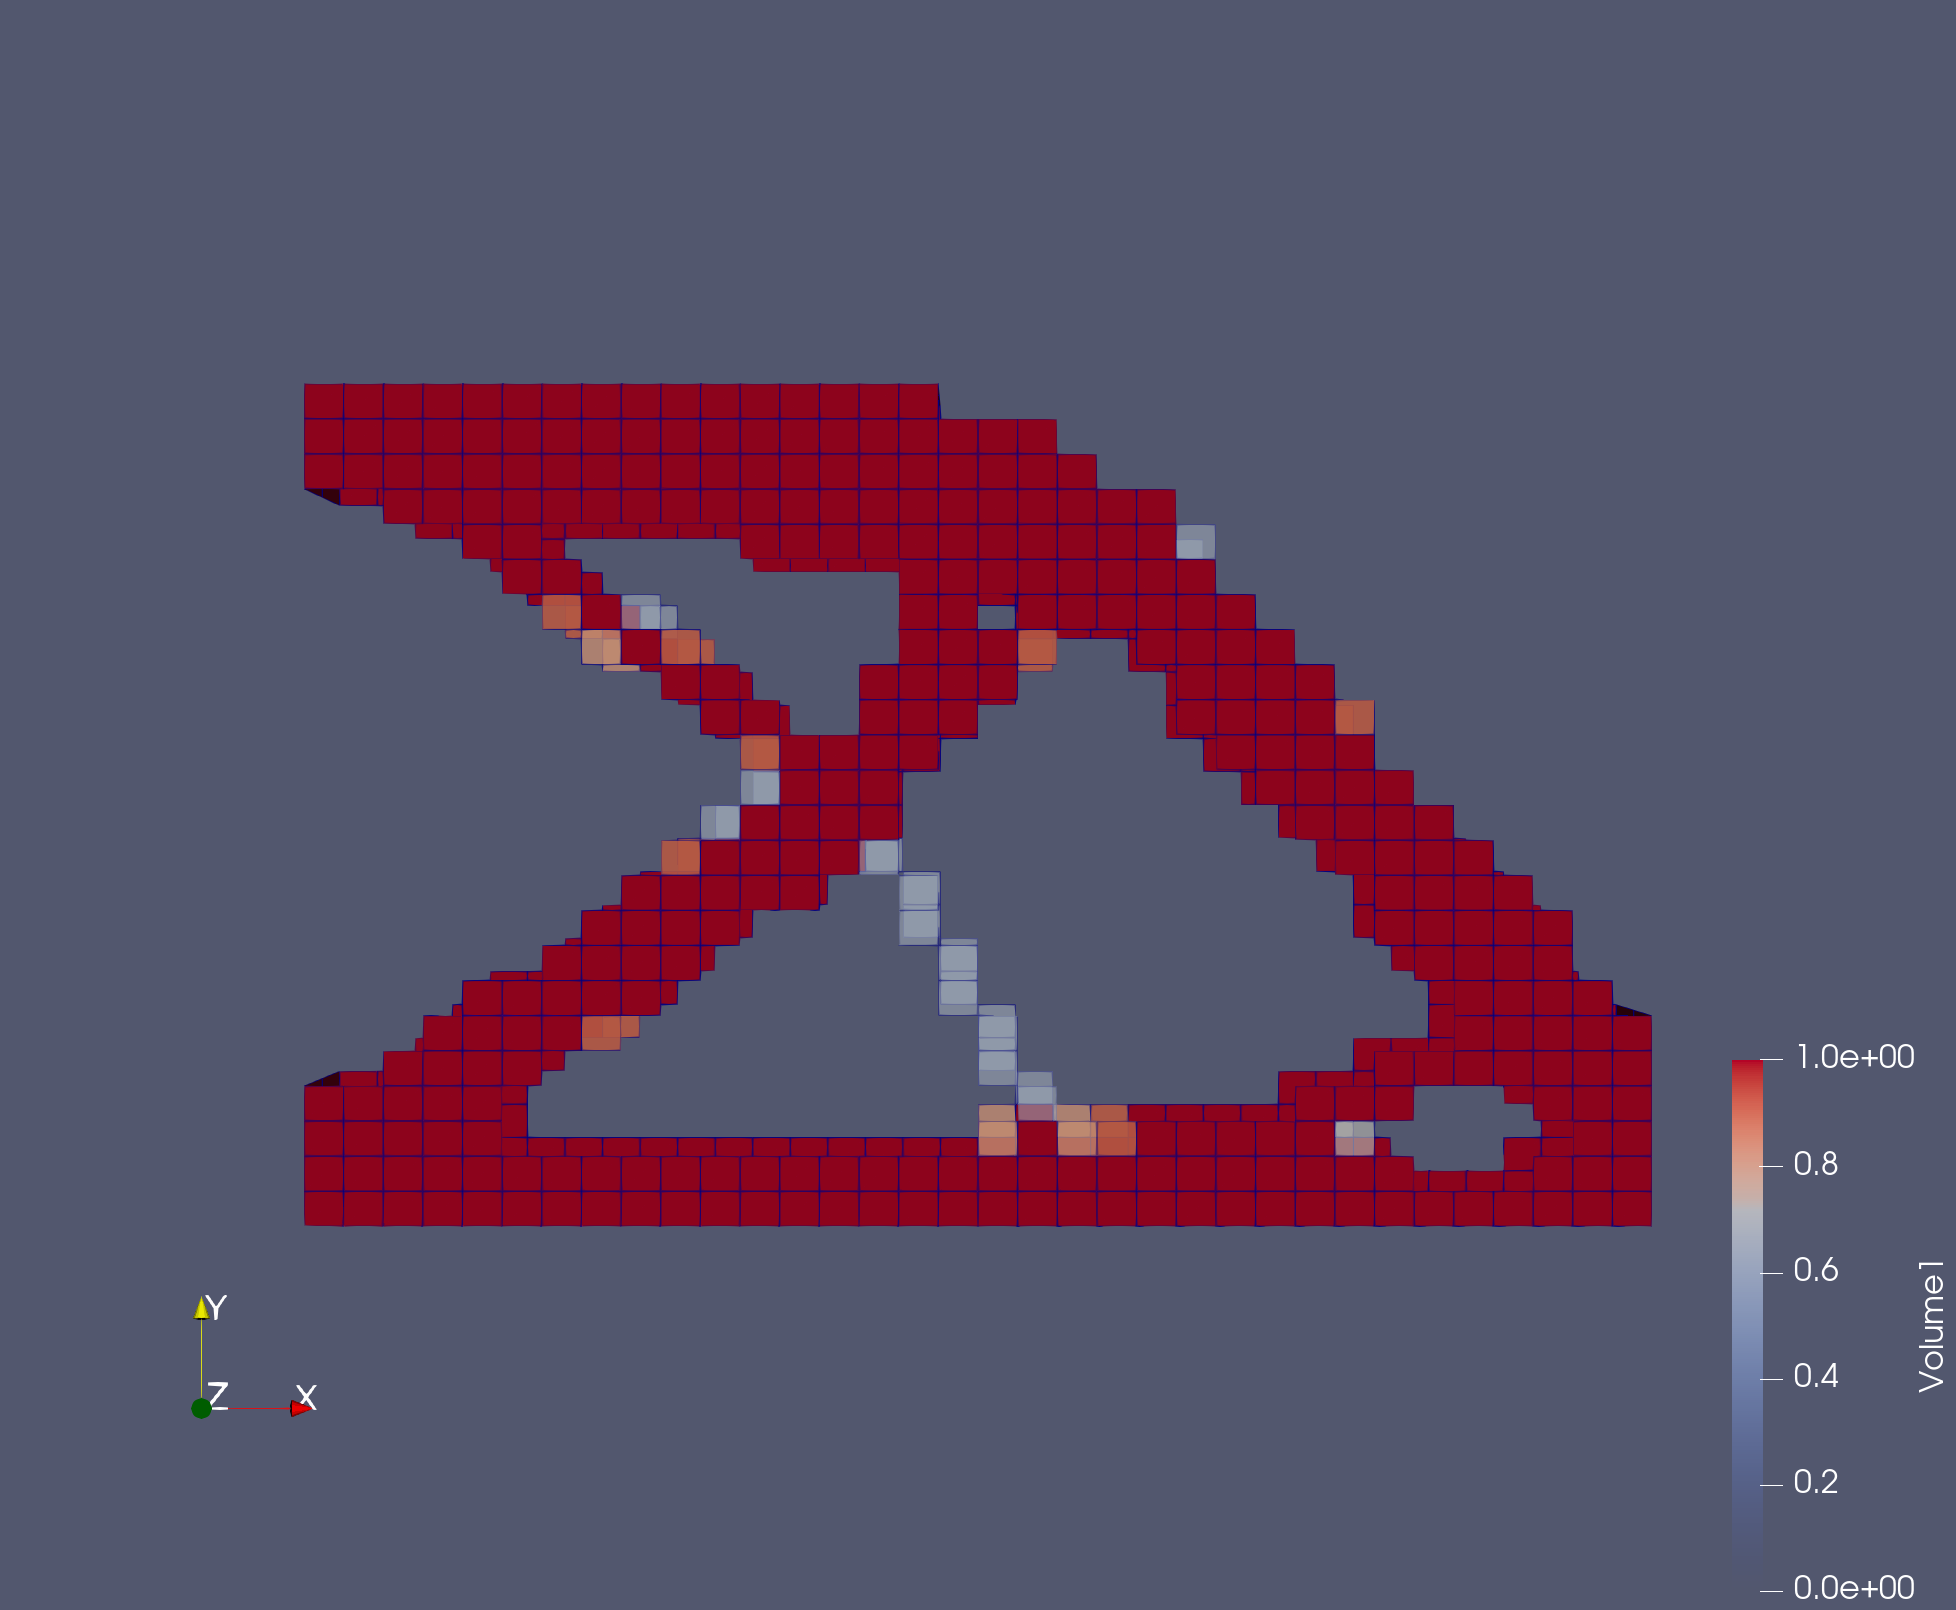
\includegraphics[width=1\linewidth]{Numerical_result_MMA_01.png}
		\captionof{figure}{Optimized structure using MMA method\\ 
		\textbf{Program generated result, plotted in paraview}}
		\label{VC-01.2}
	\end{minipage}
\end{figure} 


\begin{figure}[H]
\centering
\includegraphics[width=1\linewidth]{Numerical_result_full_MMA_01.jpg}
\centering
\caption{Topology optimized structure of cantilever beam with volume fraction 0.4, penalty 3 and rmin 1.5, plotted using pyvista}
\label{VC-01.3}
\end{figure}
\begin{figure}[H]
\centering
\includegraphics[width=0.85\linewidth]{Compliance_chg_MMA_01.png}
\centering
\caption{Change of compliance at every iteration, plotted structure at 1,10,40 and last iterations}

\label{VC-01.4}
\end{figure}
\begin{figure}[H]
	\centering
	\begin{minipage}{.5\textwidth}
		\centering
		\includegraphics[width=1\linewidth]{MMA_01_discretness.png}
		\captionof{figure}{Mesaure of discretness }
		\label{VC-01.5}
	\end{minipage}%
	\begin{minipage}{.5\textwidth}
		\centering
		\includegraphics[width=1\linewidth]{MMA_01_Volume_fractionVSiteration.png}
		\captionof{figure}{Change in volume fraction at each iteration}
		\label{VC-01.6}
	\end{minipage}
\end{figure} 
\subsubsection{Problem solved using OC optimizer}
Cantilever beam with load at free end with density 7850 kg/m$^3$. The problem is solved using optimality criteria method to get optimized structure. The following list can be used to obtain the below results.\\
\begin{lstlisting}
INPUTS:
8 5 1 35 25 3 -100 0.4 3 1.5 150000 0.35 7850 0 0 1
\end{lstlisting}
The comparison of the results from literature$^{\citep{ISOtop}}$ and program generated optimized structure is done in figure (\ref{VC-02.1}) and (\ref{VC-02.2}).\\
The change in the structure and it's compliance are plotted at regular intervals in figure (\ref{VC-02.4}) and change in volume fraction at each iteration is plotted in figure (\ref{VC-02.5}).\\
Measure of discretness- The number of elements which are in the between 0 and 1 as shown in figure (\ref{VC-02.6}).\\
 
\begin{figure}[H]
	\centering
	\begin{minipage}{.5\textwidth}
		\centering
		\includegraphics[width=1\linewidth]{analytical_OC_1.png}
		\captionof{figure}{IGTO validation-1 for OC
			\\\textbf{Results from literature}\citep{ISOtop}}
		\label{VC-02.1}
	\end{minipage}%
	\begin{minipage}{.5\textwidth}
		\centering
		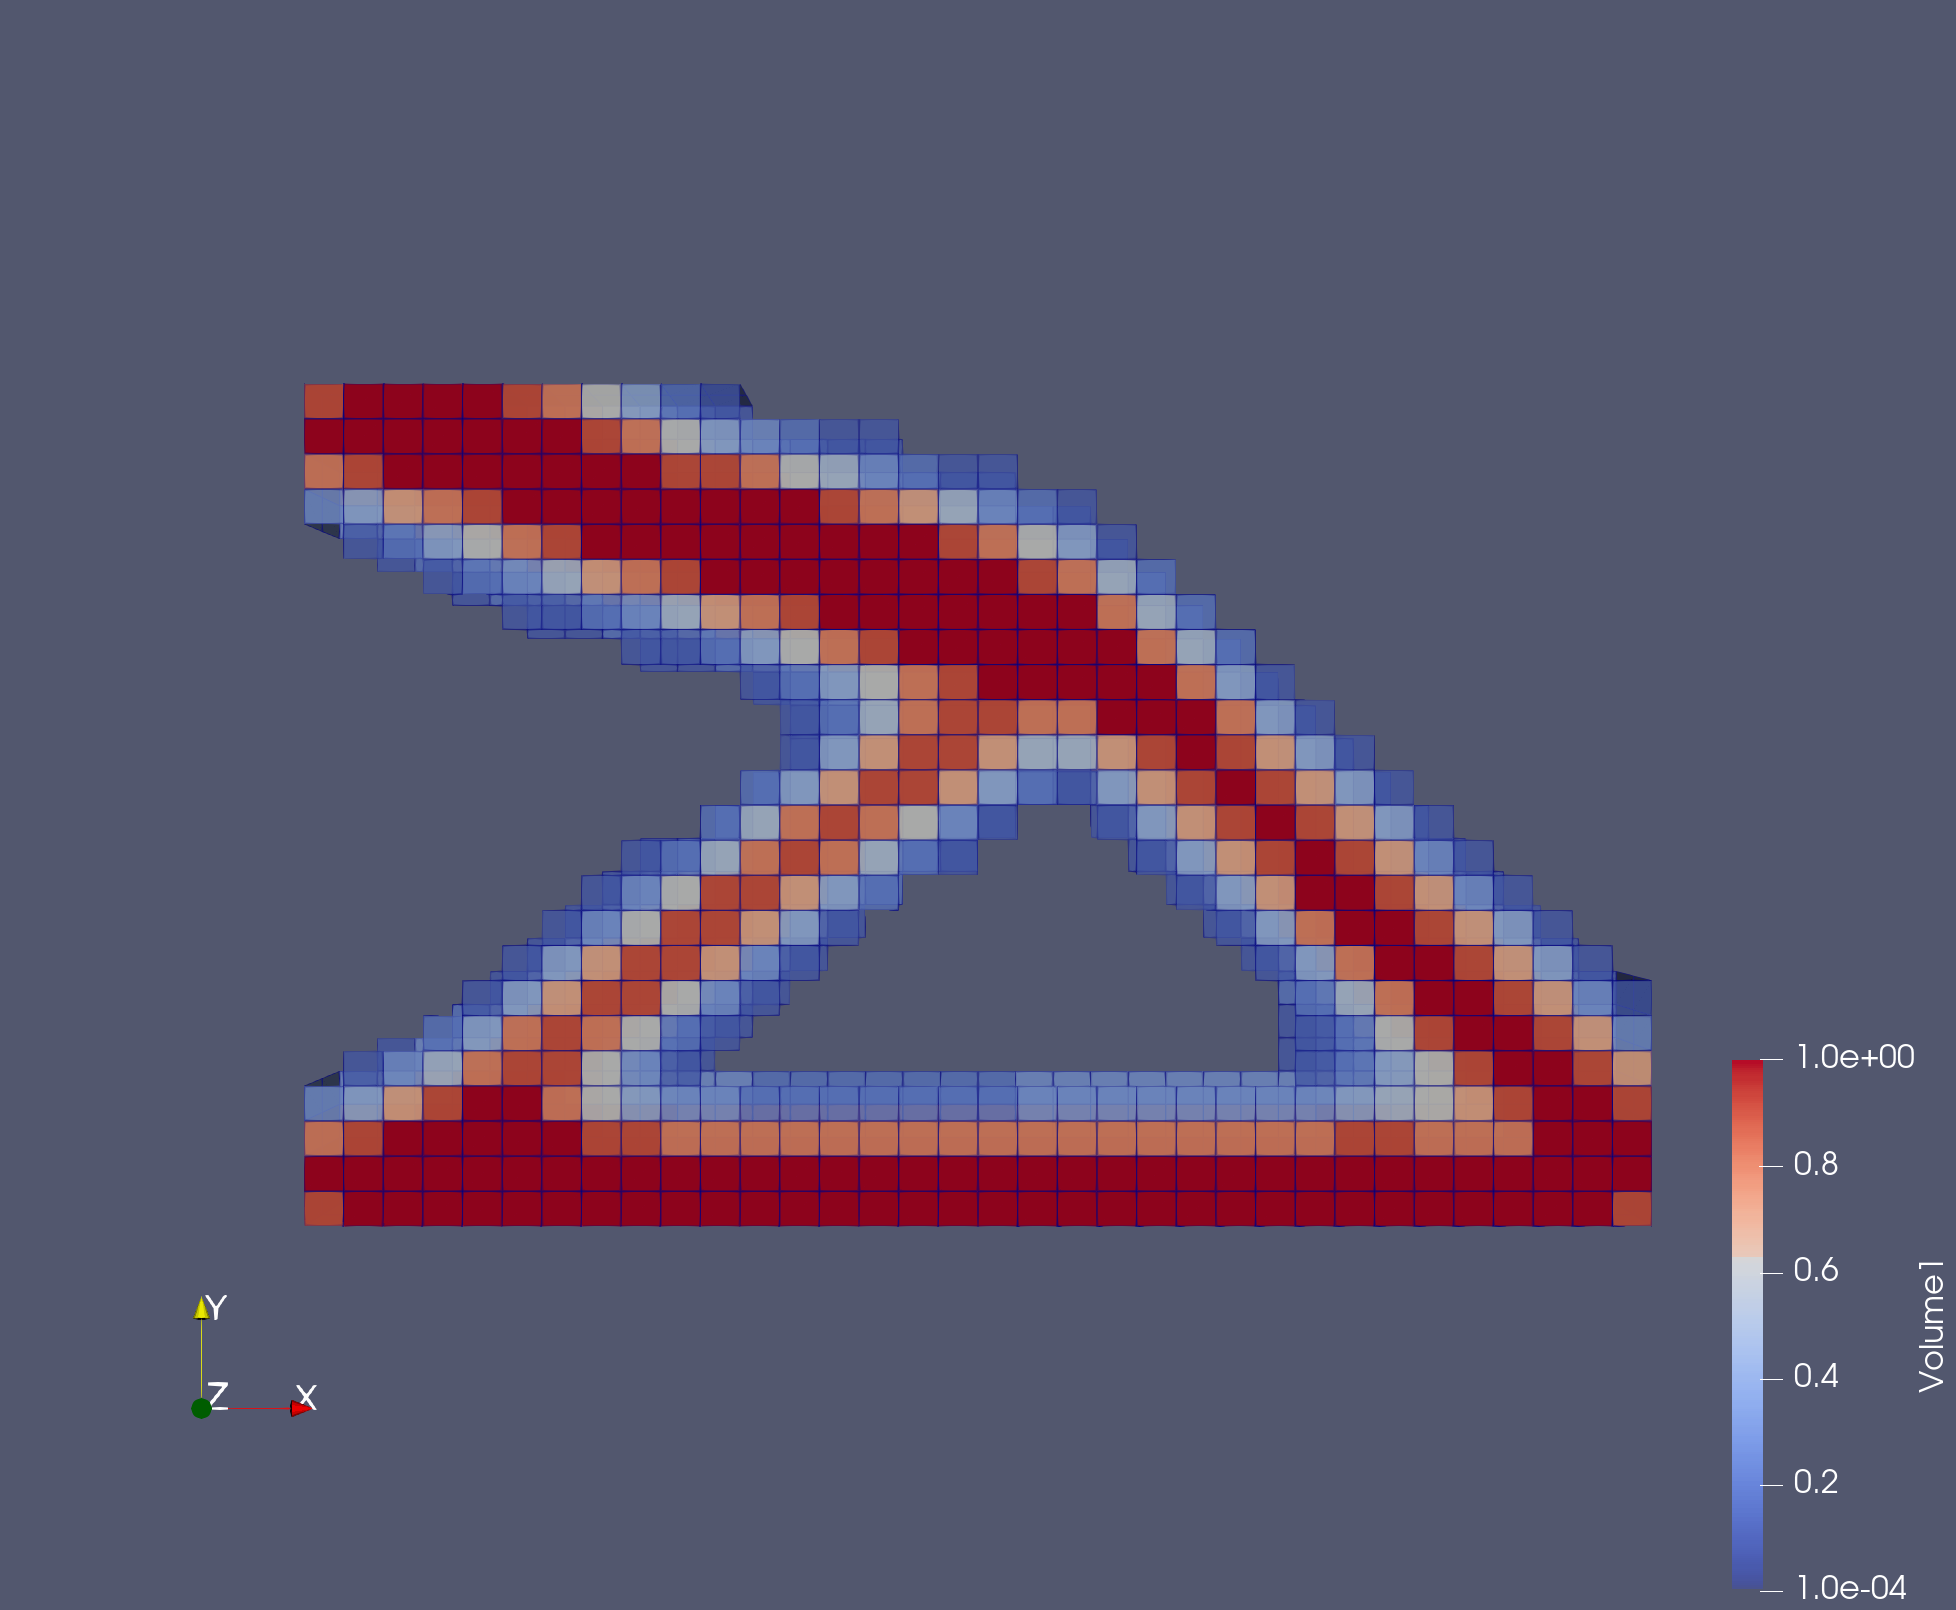
\includegraphics[width=1\linewidth]{Numerical_result_OC_01.png}
		\captionof{figure}{Optimized structure using OC method\\ 
		\textbf{Program generated result, plotted in paraview}}
		\label{VC-02.2}
	\end{minipage}
\end{figure} 
\begin{figure}[H]
	\centering
	\begin{minipage}{.5\textwidth}
		\centering
		\includegraphics[width=1\linewidth]{OC_01_discretness.png}
		\captionof{figure}{Mesaure of discretness }
		\label{VC-02.5}
	\end{minipage}%
	\begin{minipage}{.5\textwidth}
		\centering
		\includegraphics[width=1\linewidth]{OC_01_Volume_fractionVSiteration.png}
		\captionof{figure}{Change in volume fraction at each iteration}
		\label{VC-02.6}
	\end{minipage}
\end{figure} 

\begin{figure}[H]
\centering
\includegraphics[width=1\linewidth]{Numerical_result_full_OC_01.jpg}
\centering
\caption{Topology optimized structure of cantilever beam with volume fraction 0.4, penalty 3 and rmin 1.5 plotted using pyvista}
\label{VC-02.3}
\end{figure}
\begin{figure}[H]
\centering
\includegraphics[width=1\linewidth]{Compliance_chg_OC_01.png}
\centering
\caption{Change of compliance at every iteration, plotted structure at 1,40,100,160 and last iterations}

\label{VC-02.4}
\end{figure}
\subsubsection{Results discussion}
\begin{enumerate}
\item Lower compliance is achieved using MMA and the number of iterations required to achieve optimized structure are less using MMA than OC method.

\item From figure (\ref{VC-01.1}) and (\ref{VC-01.2}), a slight deviation from the original solution can be accounted to the dependency of optimized structure on number of elements and comparison of 2d structure results from paper with program results obtained from 3D analysis.

\item The measure of discreteness for MMA and OC methods shows that MMA penalizes the element volume effectively than OC method.

\item From volume fraction change at each iteration for MMA and OC methods. As MMA is gradient based method it approaches the final volume gradually where as OC is penalty based method therefore fluctuates about the volume constraint.
\end{enumerate}

\end{subsection}


\begin{subsection}{Validation test case-2}
\subsubsection{Problem description}
A simple support beam is subjected to load at center of the free end. As shown in figure(\ref{fig:problem-2})
\begin{figure}[H]
	\begin{center}
		\includegraphics[scale=0.5]{Problem-2.png} 
		\caption{\\Cantilever beam with load at center of the free end}\label{fig:problem-2}
	\end{center}	
\end{figure}

\subsubsection{Input parameters}
The input parameters are Length 8cm, Height 5cm, Width 1cm, Young's modulus 150000 N/m, Poisson ratio 0.3, load 100 N, volume fraction 0.4(optimized volume V/original volume V0), penalization factor 3, minimum radius 1.5 \\ 
Degree of the curve\\
p=1,q=1,r=1.

\subsubsection{Problem solved using MMA optimizer}
Cantilever beam with load at center of the free end with density 7850 kg/m$^3$. The problem is solved using Moving Asymptotes method to get optimized structure. The following list can be used to obtain the below results.\\
\begin{lstlisting}
INPUTS:
8 5 1 35 25 3 -100 0.4 5 1.5 150000 0.35 7850 5 1 1
\end{lstlisting}
The comparison of the results from literature$^{\citep{ISOtop}}$ and program generated optimized structure is done in figure (\ref{VC-03.1}) and (\ref{VC-03.2}).\\
The change in the structure and it's compliance are plotted at regular intervals in figure (\ref{VC-03.4}) and change in volume fraction at each iteration is plotted in figure (\ref{VC-03.5}).\\
Measure of discretness- The number of elements which are in the between 0 and 1 as shown in figure (\ref{VC-03.6}).\\
 
\begin{figure}[H]
	\centering
	\begin{minipage}{.5\textwidth}
		\centering
		\includegraphics[width=1\linewidth]{analytical_OC_2.png}
		\captionof{figure}{IGTO validation-2 for MMA
			\\\textbf{Results from literature}\citep{ISOtop}}
		\label{VC-03.1}
	\end{minipage}%
	\begin{minipage}{.5\textwidth}
		\centering
		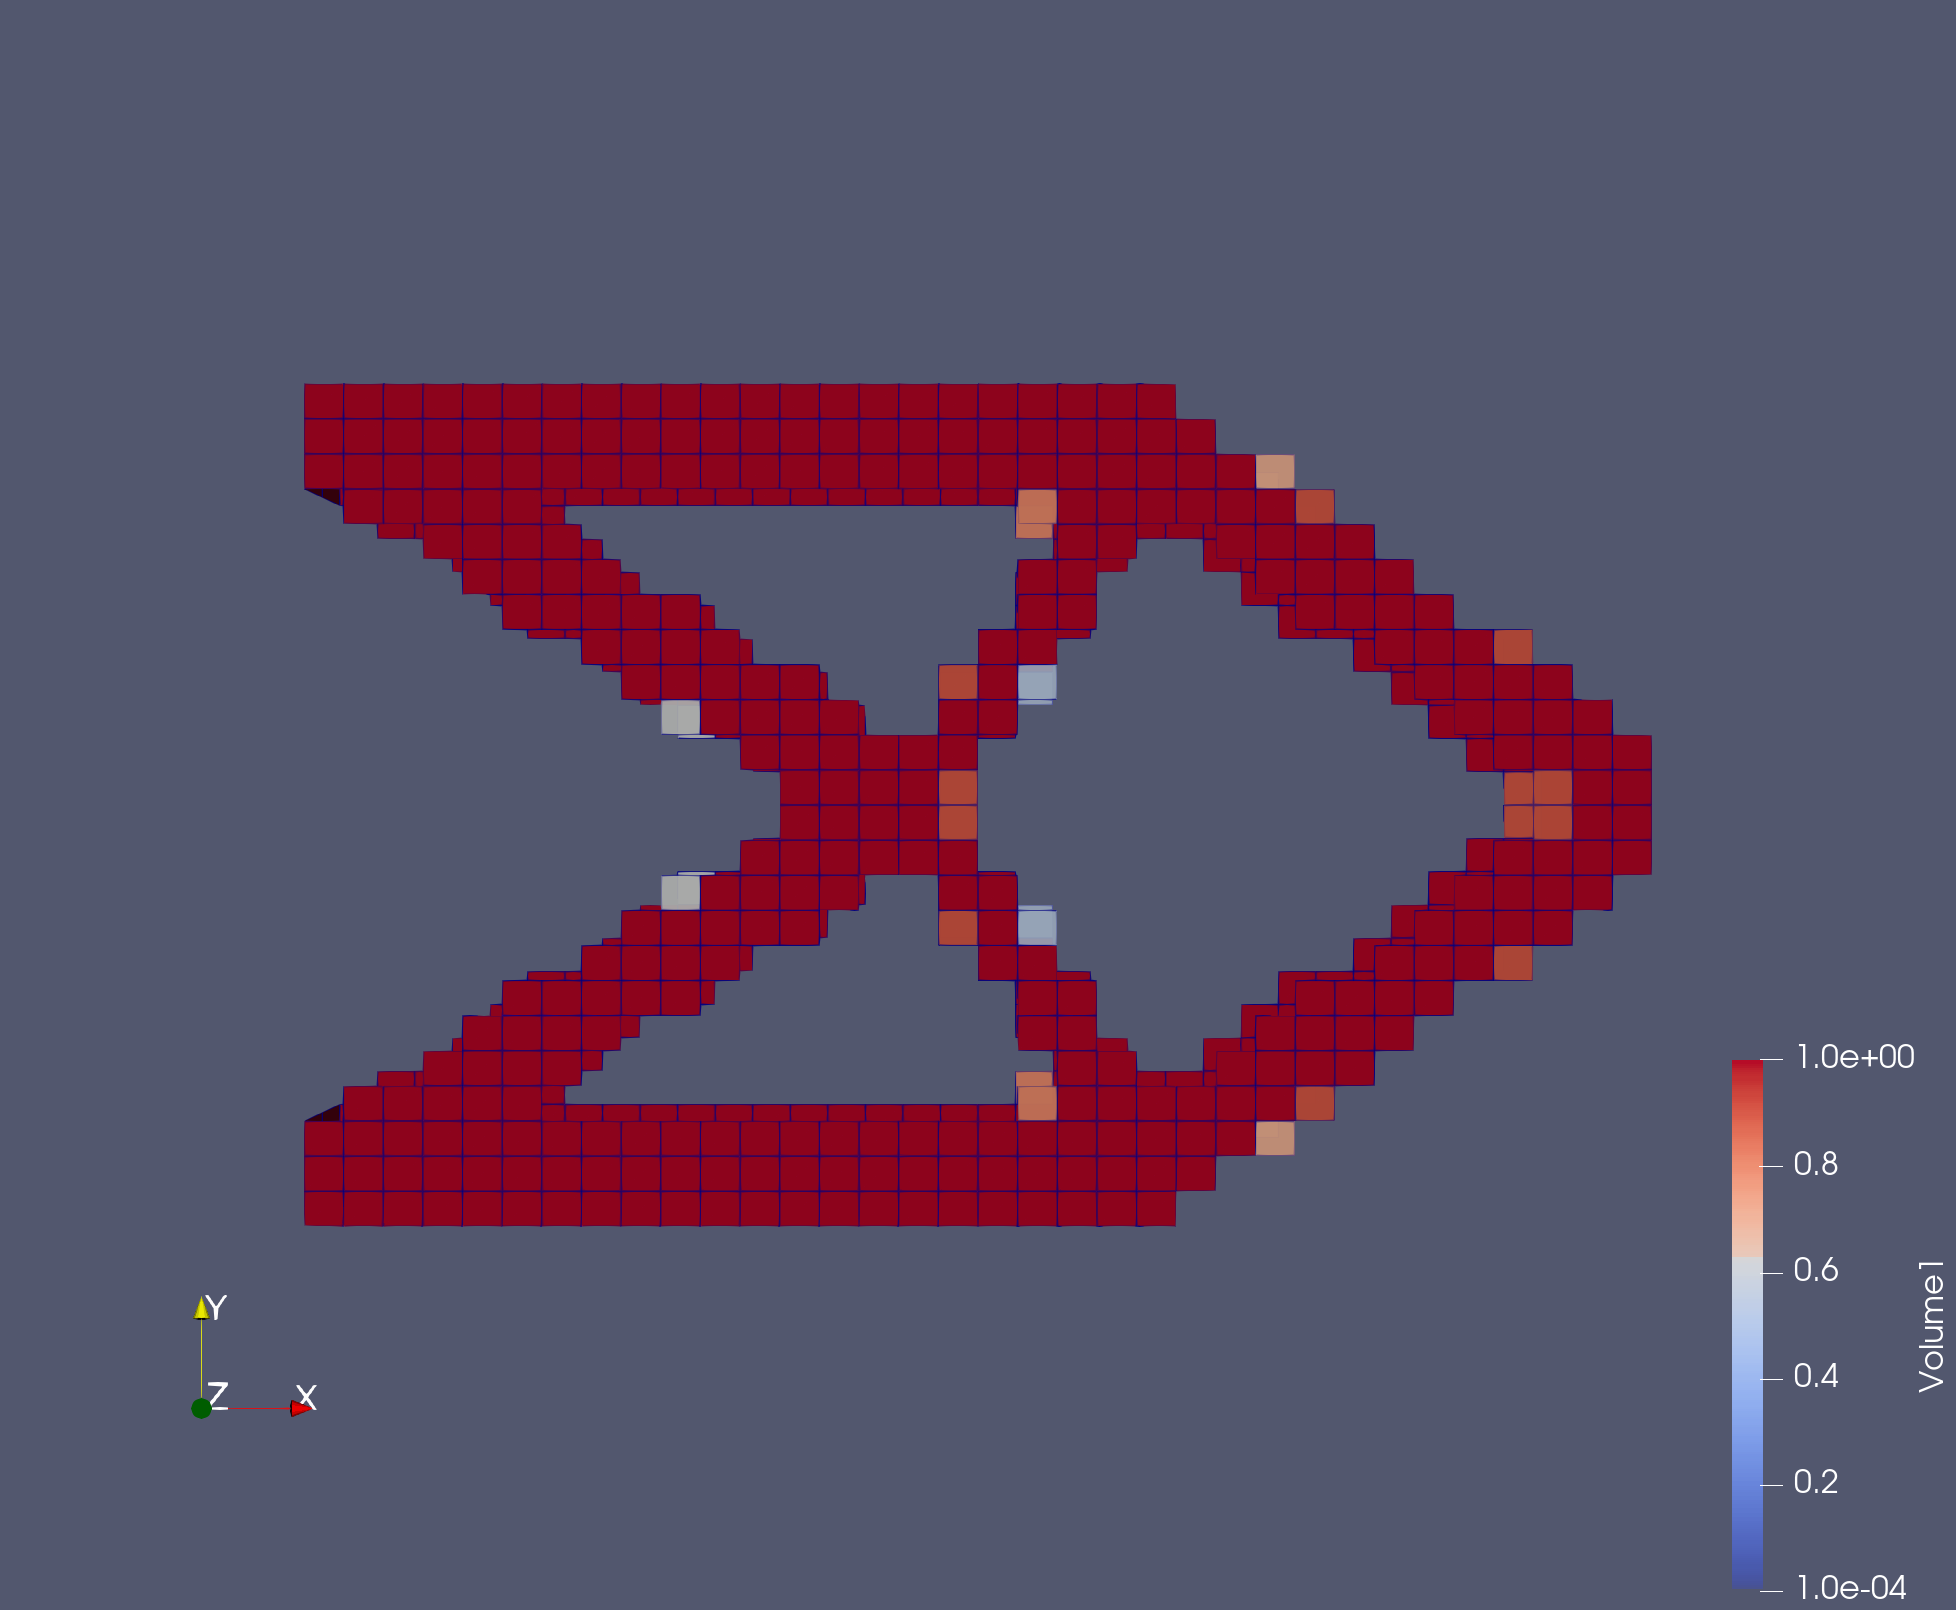
\includegraphics[width=1\linewidth]{Numerical_result_MMA_02.png}
		\captionof{figure}{Optimized structure using MMA method\\ 
		\textbf{Program generated result, plotted in paraview}}
		\label{VC-03.2}
	\end{minipage}
\end{figure} 
\begin{figure}[H]
	\centering
	\begin{minipage}{.5\textwidth}
		\centering
		\includegraphics[width=1\linewidth]{MMA_02_discretness.png}
		\captionof{figure}{Mesaure of discretness }
		\label{VC-03.5}
	\end{minipage}%
	\begin{minipage}{.5\textwidth}
		\centering
		\includegraphics[width=1\linewidth]{MMA_02_Volume_fractionVSiteration.png}
		\captionof{figure}{Change in volume fraction at each iteration}
		\label{VC-03.6}
	\end{minipage}
\end{figure} 

\begin{figure}[H]
\centering
\includegraphics[width=1\linewidth]{Numerical_result_full_MMA_02.jpg}
\centering
\caption{Topology optimized structure of cantilever beam with volume fraction 0.4, penalty 3 and rmin 1.5,plotted using pyvista}
\label{VC-03.3}
\end{figure}
\begin{figure}[H]
\centering
\includegraphics[width=1\linewidth]{Compliance_chg_MMA_02.png}
\centering
\caption{Change of compliance at every iteration, plotted structure at 1,10,20 and last iterations}

\label{VC-03.4}
\end{figure}

\subsubsection{Problem solved using OC optimizer}
Cantilever beam with load at center of the free end with density 7850 kg/m$^3$. The problem is solved using optimality criteria method to get optimized structure. The following list can be used to obtain the below results.\\
\begin{lstlisting}
INPUTS:
8 5 1 35 25 3 -100 0.4 3 1.5 150000 0.35 7850 5 0 1
\end{lstlisting}
The comparison of the results from literature$^{\citep{ISOtop}}$ and program generated optimized structure is done in figure (\ref{VC-04.1}) and (\ref{VC-04.2}).\\
The change in the structure and it's compliance are plotted at regular intervals in figure (\ref{VC-04.4}) and change in volume fraction at each iteration is plotted in figure (\ref{VC-04.6}).\\
Measure of discretness- The number of elements which are in the between 0 and 1 as shown in figure (\ref{VC-04.5}).\\
 
\begin{figure}[H]
	\centering
	\begin{minipage}{.5\textwidth}
		\centering
		\includegraphics[width=1\linewidth]{analytical_OC_2.png}
		\captionof{figure}{IGTO validation-2 for OC
			\\\textbf{Results from literature}\citep{ISOtop}}
		\label{VC-04.1}
	\end{minipage}%
	\begin{minipage}{.5\textwidth}
		\centering
		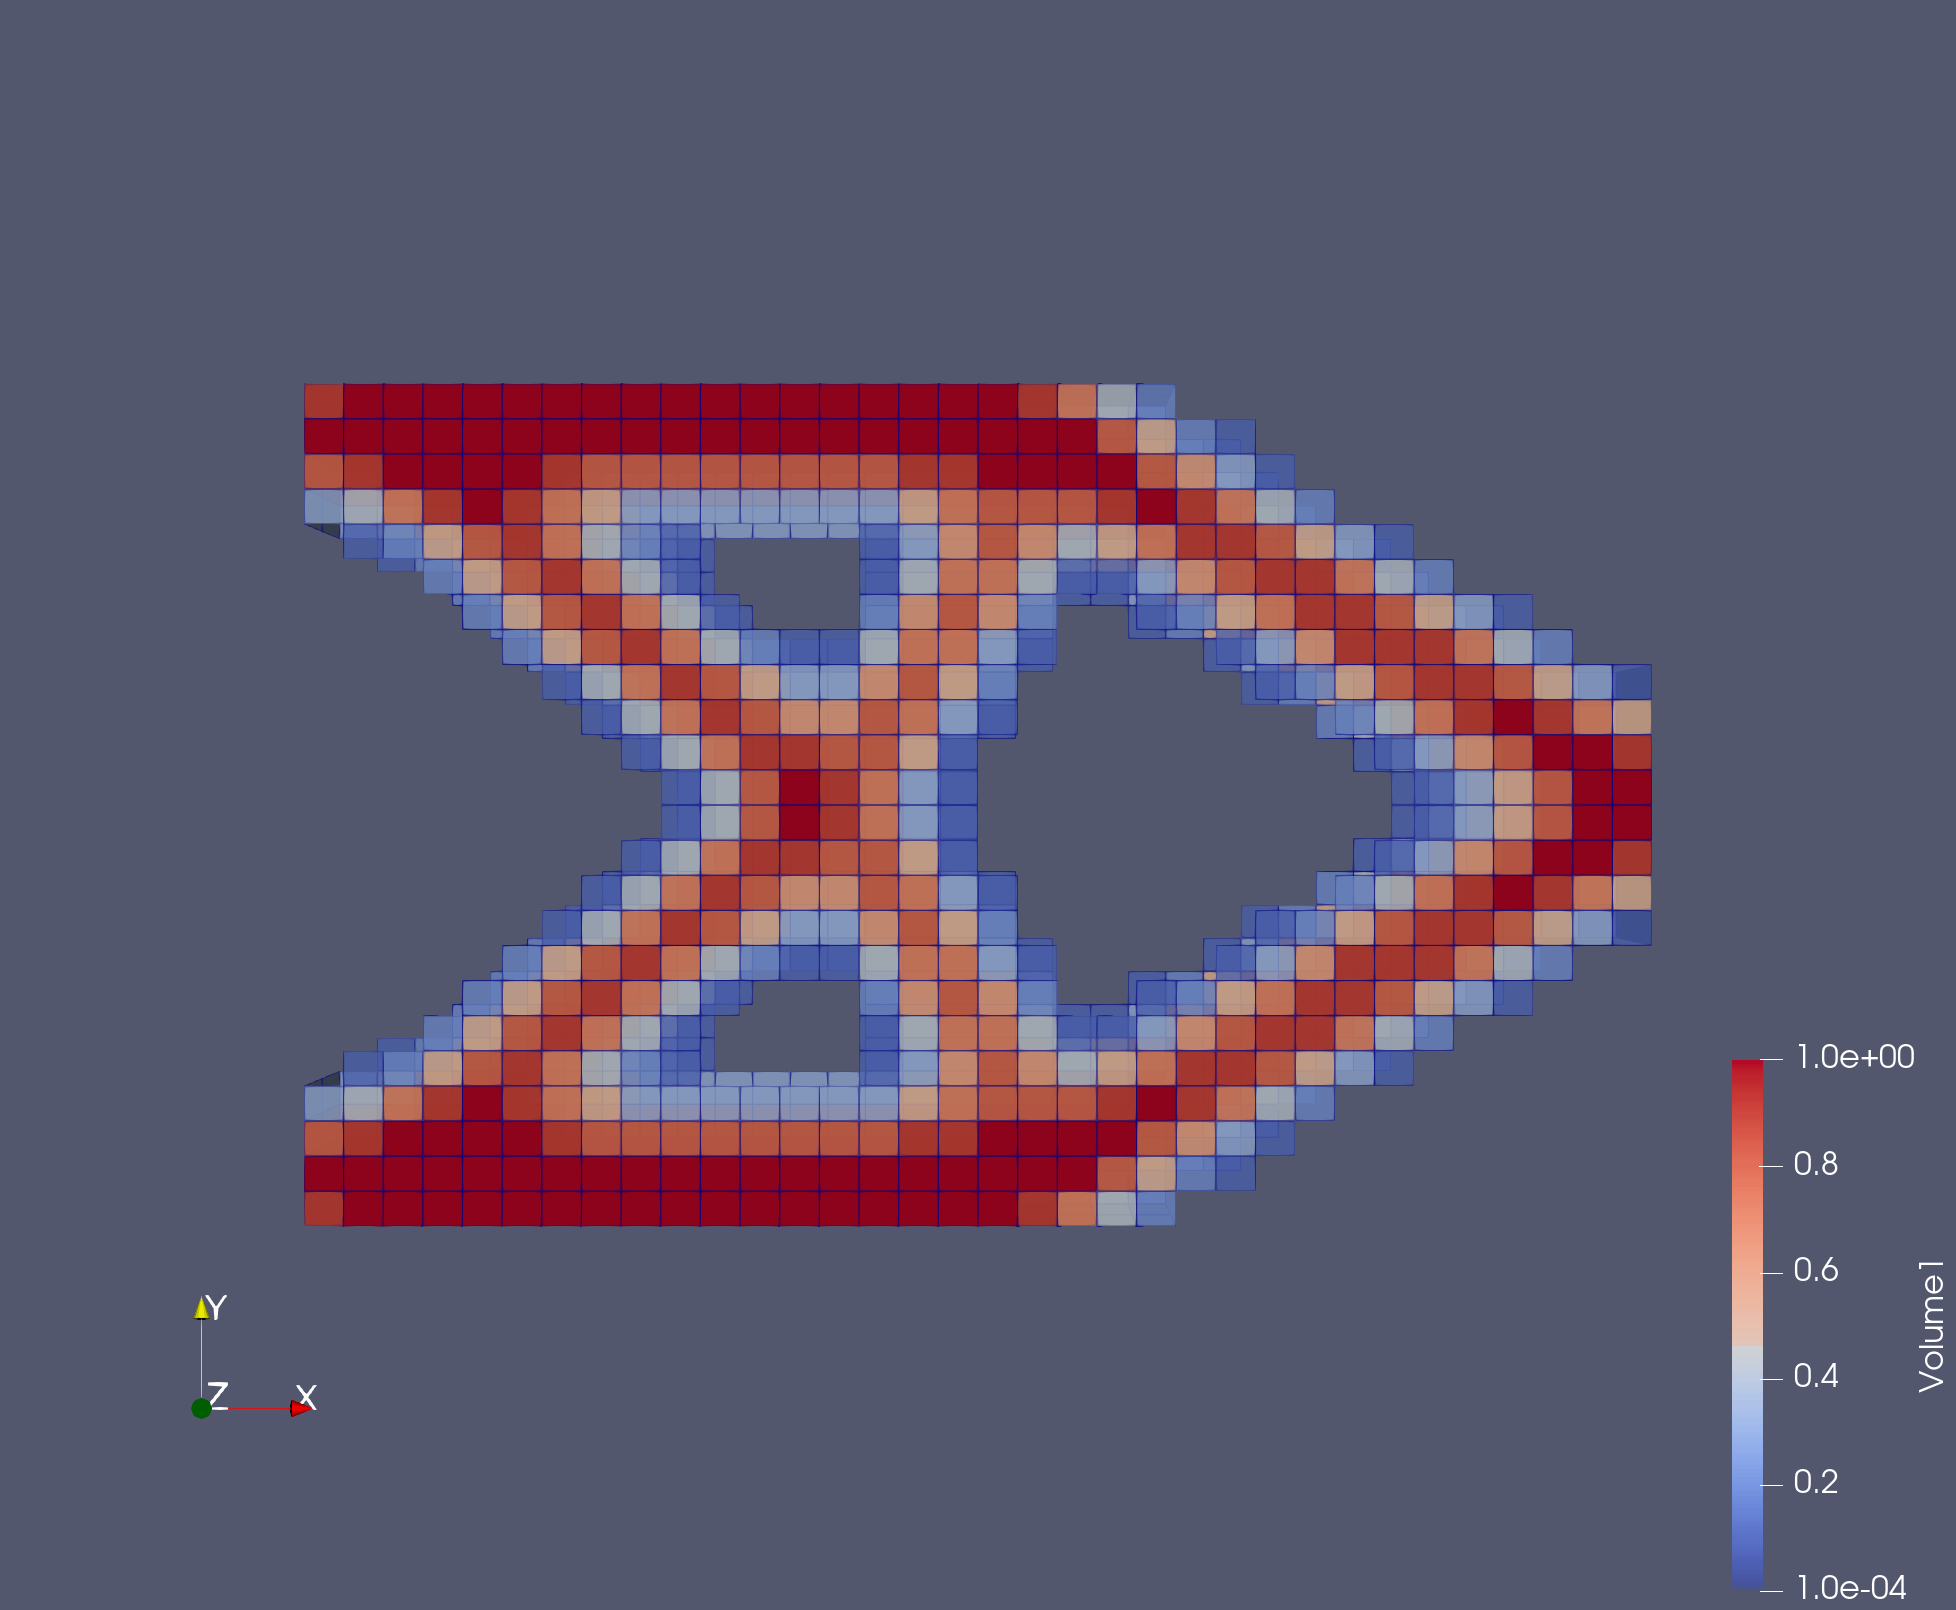
\includegraphics[width=1\linewidth]{Numerical_result_OC_02.png}
		\captionof{figure}{Optimized structure using OC method\\ 
		\textbf{Program generated result, plotted in paraview}}
		\label{VC-04.2}
	\end{minipage}
\end{figure} 
\begin{figure}[H]
	\centering
	\begin{minipage}{.5\textwidth}
		\centering
		\includegraphics[width=1\linewidth]{OC_02_discretness.png}
		\captionof{figure}{Mesaure of discretness }
		\label{VC-04.5}
	\end{minipage}%
	\begin{minipage}{.5\textwidth}
		\centering
		\includegraphics[width=1\linewidth]{OC_02_Volume_fractionVSiteration.png}
		\captionof{figure}{Change in volume fraction at each iteration}
		\label{VC-04.6}
	\end{minipage}
\end{figure} 

\begin{figure}[H]
\centering
\includegraphics[width=1\linewidth]{Numerical_result_full_OC_02.jpg}
\centering
\caption{Topology optimized structure of cantilever beam with volume fraction 0.4, penalty 3 and rmin 1.5,plotted using pyvista}
\label{VC-04.3}
\end{figure}
\begin{figure}[H]
\centering
\includegraphics[width=1\linewidth]{Compliance_chg_OC_02.png}
\centering
\caption{Change of compliance at every iteration, plotted structure at 1,10,60,100 and last iterations}
\label{VC-04.4}
\end{figure}
\subsubsection{Results discussion}
\begin{enumerate}
\item Lower compliance is achieved using MMA and the number of iterations required to achieve optimized structure are less using MMA than OC method.

\item The measure of discreteness for MMA and OC methods shows that MMA penalizes the element volume effectively than OC method.

\item From volume fraction change at each iteration for MMA and OC methods. As MMA is gradient based method it approaches the final volume gradually where as OC is penalty based method therefore fluctuates about the volume constraint.

\item The convergence to optimal solution using OC method is not efficient which can be improved by using filters.
\end{enumerate}

\end{subsection}


\begin{subsection}{Validation test case-3}
\subsubsection{Problem description}
A Simple supported beam is subject to load at center. As shown in figure(\ref{fig:problem-3})
\begin{figure}[H]
	\begin{center}
		\includegraphics[scale=0.5]{Problem-3.png} 
		\caption{\\Simple supported beam with load at center}\label{fig:problem-3}
	\end{center}	
\end{figure}

\subsubsection{Input parameters}
The input parameters are Length 8cm, Height 5cm, Width 1cm, Young's modulus 150000 N/m, Poisson ratio 0.3, load 100 N, volume fraction 0.4(optimized volume V/original volume V0), penalization factor 3, minimum radius 1.5 \\ 
Degree of the curve\\
p=1,q=1,r=1.

\subsubsection{Problem solved using MMA optimizer}
Simple supported beam with load at center with density 7850 kg/m$^3$. The problem is solved using Moving Asymptotes method to get optimized structure. The following list can be used to obtain the below results.\\
\begin{lstlisting}
INPUTS:
8 5 1 35 25 3 -100 0.2 3 1.5 150000 0.35 7850 1 1 1
\end{lstlisting}
The comparison of the results from literature$^{\citep{ISOtop}}$ and program generated optimized structure is done in figure (\ref{VC-05.1}) and (\ref{VC-05.2}).\\
The change in the structure and it's compliance are plotted at regular intervals in figure (\ref{VC-05.4}) and change in volume fraction at each iteration is plotted in figure (\ref{VC-05.5}).\\
Measure of discretness- The number of elements which are in the between 0 and 1 as shown in figure (\ref{VC-05.6}).\\
 
\begin{figure}[H]
	\centering
	\begin{minipage}{.5\textwidth}
		\centering
		\includegraphics[width=1\linewidth]{analytical_3.png}
		\captionof{figure}{IGTO validation-3 for MMA
			\\\textbf{Results from literature}\citep{ISOtop}}
		\label{VC-05.1}
	\end{minipage}%
	\begin{minipage}{.5\textwidth}
		\centering
		\includegraphics[width=1\linewidth]{Numerical_result_MMA_03.png}
		\captionof{figure}{Optimized structure using MMA method\\ 
		\textbf{Program generated result, plotted in paraview}}
		\label{VC-05.2}
	\end{minipage}
\end{figure} 
\begin{figure}[H]
	\centering
	\begin{minipage}{.5\textwidth}
		\centering
		\includegraphics[width=1\linewidth]{MMA_03_discretness.png}
		\captionof{figure}{Mesaure of discretness }
		\label{VC-05.5}
	\end{minipage}%
	\begin{minipage}{.5\textwidth}
		\centering
		\includegraphics[width=1\linewidth]{MMA_03_Volume_fractionVSiteration.png}
		\captionof{figure}{Change in volume fraction at each iteration}
		\label{VC-05.6}
	\end{minipage}
\end{figure} 

\begin{figure}[H]
\centering
\includegraphics[width=1\linewidth]{Numerical_result_full_MMA_03.jpg}
\centering
\caption{Topology optimized structure of cantilever beam with volume fraction 0.2, penalty 3 and rmin 1.5,plotted using pyvista}
\label{VC-05.3}
\end{figure}
\begin{figure}[H]
\centering
\includegraphics[width=1\linewidth]{Compliance_chg_MMA_03.png}
\centering
\caption{Change of compliance at every iteration, plotted structure at 1,10,40 and last iterations}

\label{VC-05.4}
\end{figure}

\subsubsection{Problem solved using OC optimizer}
Simple supported beam with load at center with density 7850 kg/m$^3$. The problem is solved using optimality criteria method to get optimized structure. The following list can be used to obtain the below results.\\
\begin{lstlisting}
INPUTS:
8 5 1 35 25 3 -100 0.2 3 1.5 150000 0.35 7850 1 0 1
\end{lstlisting}
The comparison of the results from literature$^{\citep{ISOtop}}$ and program generated optimized structure is done in figure (\ref{VC-06.1}) and (\ref{VC-06.2}).\\
The change in the structure and it's compliance are plotted at regular intervals in figure (\ref{VC-06.4}) and change in volume fraction at each iteration is plotted in figure (\ref{VC-06.6}).\\
Measure of discretness- The number of elements which are in the between 0 and 1 as shown in figure (\ref{VC-06.5}).\\
 
\begin{figure}[H]
	\centering
	\begin{minipage}{.5\textwidth}
		\centering
		\includegraphics[width=1\linewidth]{analytical_3.png}
		\captionof{figure}{IGTO validation-3 for OC
			\\\textbf{Results from paper}\citep{ISOtop}}
		\label{VC-06.1}
	\end{minipage}%
	\begin{minipage}{.5\textwidth}
		\centering
		\includegraphics[width=1\linewidth]{Numerical_result_OC_03.png}
		\captionof{figure}{Optimized structure using OC method\\ 
		\textbf{Program generated result, plotted in paraview}}
		\label{VC-06.2}
	\end{minipage}
\end{figure} 
\begin{figure}[H]
	\centering
	\begin{minipage}{.5\textwidth}
		\centering
		\includegraphics[width=1\linewidth]{OC_03_discretness.png}
		\captionof{figure}{Mesaure of discretness }
		\label{VC-06.5}
	\end{minipage}%
	\begin{minipage}{.5\textwidth}
		\centering
		\includegraphics[width=1\linewidth]{OC_03_Volume_fractionVSiteration.png}
		\captionof{figure}{Change in volume fraction at each iteration}
		\label{VC-06.6}
	\end{minipage}
\end{figure} 

\begin{figure}[H]
\centering
\includegraphics[width=1\linewidth]{Numerical_result_full_OC_03.jpg}
\centering
\caption{Topology optimized structure of cantilever beam with volume fraction 0.2, penalty 3 and rmin 1.5, plotted using pyvista}
\label{VC-06.3}
\end{figure}
\begin{figure}[H]
\centering
\includegraphics[width=1\linewidth]{Compliance_chg_OC_03.png}
\centering
\caption{Change of compliance at every iteration, plotted structure at 1,10,60,180 and last iterations}
\label{VC-06.4}
\end{figure}
\subsubsection{Results discussion}
\begin{enumerate}
\item Lower compliance is achieved using MMA and the number of iterations required to achieve optimized structure are less using MMA than OC method.

\item The discrepancy in results for both MMA and OC method is because of the 2D analysis is performed in the literature which could account for the straining along z direction.

\item The measure of discreteness for MMA and OC methods shows that MMA penalizes the element volume effectively than OC method.

\item From volume fraction change at each iteration for MMA and OC methods. As MMA is gradient based method it approaches the final volume gradually where as OC is penalty based method therefore fluctuates about the volume constraint.

\item The convergence to optimal solution using OC method is not efficient which can be improved by using filters.
\end{enumerate}

\end{subsection}
\begin{subsection}{Influence of parameters on topology optimization}
\subsubsection{Problem statement}
A cantilever beam is subject to load at the free end. As shown in figure -\ref{fig:problem-1}
\begin{figure}[H]
	\begin{center}
		\includegraphics[scale=1.75]{Problem-1.png} 
		\caption{\\Cantilever beam with load at free end}\label{fig:problem-1}
	\end{center}	
\end{figure}


\subsubsection{Penalization factor}
Inputs are same as in validation case-1. Penalization factor is used to remove porosity with in material so checker board pattern can be avoided. 
The change in topology optimization based on the penalization factor \textbf{P} is shown in Table-\ref{table:1}. \\
rmin is constant 1.5 and {P} is changed.
\begin{lstlisting}
INPUTS:
8 5 1 35 25 3 -100 0.4 {P} 1.5 150000 0.35 7850 0 1 1
\end{lstlisting}

\begin{center} 
\begin{table} [H]
\begin{tabular}{c|c|c} 
P & optimized structure& Discreteness of volume\\ 
\\\hline\\
5&\includegraphics[scale = 0.5]{penal_5.png} & \includegraphics[scale = 0.4]{MMA_discretness_penal_5.png}\\ 
\\\hline\\ 
10&\includegraphics[scale = 0.5]{penal_10.png} & \includegraphics[scale = 0.4]{MMA_discretness_penal_10.png}\\ 
\\\hline\\ 
20&\includegraphics[scale = 0.5]{penal_20.png} & \includegraphics[scale = 0.4]{MMA_discretness_penal_20.png}\\
\\\hline\\ 
30&\includegraphics[scale = 0.5]{penal_30.png} & \includegraphics[scale = 0.4]{MMA_discretness_penal_30.png}\\ 
\end{tabular} 
\caption{Influence of penalization factor} 
\label{table:1} 
\end{table} 
\end{center}
\subsubsection{Minimum radius (rmin) factor}
Inputs are same as in validation case-1. rmin is the minimum distance between the neighbouring elements which is used as a parameter in sensitivity analysis to build weight factor. 
The change in topology optimization based on the  \textbf{rmin} factor is shown in Table-\ref{table:2}. \\
P is constant and {rmin} is changed.
\begin{lstlisting}
INPUTS:
8 5 1 35 25 3 -100 0.4 3.5 {rmin} 150000 0.35 7850 0 1 1
\end{lstlisting}
\subsubsection{Results discussion}
\begin{enumerate}
\item The topology optimization depends mainly on penalization factor \textbf{P} and minimum radius \textbf{rmin}.
\item The influence of penalization factor on topology optimization is more elements with intermediate value are penalized. As the value of \textbf{P} increases the discreteness decreases. The value of \textbf{P} has less influence on the compliance and structure would remain relatively same.As shown in table \ref{table:1}.
\item The \textbf{rmin} value has great influence on the structure and the shape of the structure changes with \textbf{rmin}. Due to the change in structure, the compliance also changes with \textbf{rmin}. As shown in table \ref{table:2}
\item Topology optimization also depends on the type of optimizer being used like OC and MMA
\item MMA would converge faster and has less discrete  volume.
\item OC needs more number of iteration to reach optimal solution and has more discrete volume.


\end{enumerate}
\begin{center} 
\begin{table} [H]
\begin{tabular}{c|c|c} 
rmin & Optimized structure& Compliance of the structure\\ 
\\\hline\\
2&\includegraphics[scale = 0.5]{rmin_2.png} & \includegraphics[scale = 0.4]{MMA_ComplianceVSiteration_rmin_2.png}\\ 
\\\hline\\ 
5&\includegraphics[scale = 0.5]{rmin_5.png} & \includegraphics[scale = 0.4]{MMA_ComplianceVSiteration_rmin_5.png}\\ 
\\\hline\\ 
8&\includegraphics[scale = 0.5]{rmin_8.png} & \includegraphics[scale = 0.4]{MMA_ComplianceVSiteration_rmin_8.png}\\
\\\hline\\ 
15&\includegraphics[scale = 0.5]{rmin_15.png} & \includegraphics[scale = 0.4]{MMA_ComplianceVSiteration_rmin_15.png}\\ 
\end{tabular} 
\caption{Influence of rmin factor} 
\label{table:2} 
\end{table} 
\end{center} 

\end{subsection}
\end{section}
\begin{section}{Time Analysis: Bottleneck in code}
The main aim is to find the computation time of each function and find possible bottlenecks in IGTO. The time analysis is performed in \textbf{main$\_ $program$\_ $bottle$\_$neck.py} file, only time module is used in this analysis.\\

\subsection{Problem description}
A cantilever beam is subjected to load at the free end. As shown in figure -\ref{fig:problem-1}
\begin{figure}[H]
	\begin{center}
		\includegraphics[scale=1.75]{Problem-1.png} 
		\caption{\\Cantilever beam with load at free end}\label{fig:problem-1}
	\end{center}	
\end{figure}

\subsection{Input parameters}
The input parameters are Length 8cm, Height 5cm, Width 1cm, Young's modulus 150000 N/m, Poisson ratio 0.3, load 100 N, volume fraction 0.4(optimized volume V/original volume V0), penalization factor 3, minimum radius 1.5 \\ 
Degree of the curve\\
p=1,q=1,r=1.

\begin{lstlisting}
INPUTS:
8 5 1 35 25 3 -100 0.4 5 1.5 150000 0.35 7850 0 1 1
\end{lstlisting}

\subsection{Analysis and results discussion}
A log file is generated with contains the number of times the function was called , total time taken by the function  and average time taken by the function.\\
A separate log file is created for each optimizer. The log contains the top 5 functions with high execution time.A pie chart is plotted based on number of times the function was called as shown in fig.(\ref{Time pie chart})\\
\begin{figure}[H]
	\begin{center}
		\includegraphics[scale=1]{time_analysis_pie_chart.png} 
		\caption{Time analysis pie chart}\label{Time pie chart}
	\end{center}	
\end{figure}

\begin{lstlisting}
LOG FILE DATA:

AUTHOR : YASA VISWAMBHAR REDDY 

!# 1616605044.207525  Topology Optimization using Iso-Geometric Analysis 

Measure of discreteness:  2.1574617647058822

Final Volume of the optimised structure  : 0.40012254901960786

Mass of the beam at 100% volume          : 314000.0

Optimized mass of the beam               : 125638.48039215687

Initial Compliance without optimization  : 228.7315796089796

Final Compliance with optimization       : 26.888775237117564 

Total execution time of the whole program: 1363.7347421646118 sec 

The time taken to run Topology optimization: 1346.0096242427826 sec 

Execution time of IGA analysis at 100% volume : 11.451846837997437 

Top 5 function which have high average execution time 

 initial condition   
 strain displacement   
 unittoparametric   
 Compliance matrix   
 derbspline basis   

 +++++++++++The function are ordered in decreasing average time of execution+++++++++++ 

---------  initial condition  ---------
Total Number of time "  initial condition  " was called  53 times.
Average time taken by the "  initial condition  " function during one run 7.528179096725751e-05 seconds.
Total time taken by the "  initial condition  " function  0.0039899349212646484 seconds. 

---------  strain displacement  ---------
Total Number of time "  strain displacement  " was called  1396992 times.
Average time taken by the "  strain displacement  " function during one run 4.5424312235716175e-05 seconds.
Total time taken by the "  strain displacement  " function  63.45740079879761 seconds. 

---------  unittoparametric  ---------
Total Number of time "  unittoparametric  " was called  4190976 times.
Average time taken by the "  unittoparametric  " function during one run 3.492859296924389e-06 seconds.
Total time taken by the "  unittoparametric  " function  14.638489484786987 seconds. 

---------  Compliance matrix  ---------
Total Number of time "  Compliance matrix  " was called  174624 times.
Average time taken by the "  Compliance matrix  " function during one run 3.2285849253336587e-06 seconds.
Total time taken by the "  Compliance matrix  " function  0.5637884140014648 seconds. 

---------  derbspline basis  ---------
Total Number of time "  derbspline basis  " was called  4190976 times.
Average time taken by the "  derbspline basis  " function during one run 1.175686975079883e-05 seconds.
Total time taken by the "  derbspline basis  " function  49.27275896072388 seconds. 

---------  knot index  ---------
Total Number of time "  knot index  " was called  4190976 times.
Average time taken by the "  knot index  " function during one run 1.0294273584875391e-05 seconds.
Total time taken by the "  knot index  " function  43.14305353164673 seconds. 

---------  Moving asymptoes  ---------
Total Number of time "  Moving asymptoes  " was called  53 times.
Average time taken by the "  Moving asymptoes  " function during one run 0.5117317595571842 seconds.
Total time taken by the "  Moving asymptoes  " function  27.12178325653076 seconds. 

---------  prime dual  ---------
Total Number of time "  prime dual  " was called  424 times.
Average time taken by the "  prime dual  " function during one run 0.3181922936214591 seconds.
Total time taken by the "  prime dual  " function  134.91353249549866 seconds. 

---------  Knearestneighbours  ---------
Total Number of time "  Knearestneighbours  " was called  1 times.
Average time taken by the "  Knearestneighbours  " function during one run 0.1845073699951172 seconds.
Total time taken by the "  Knearestneighbours  " function  0.1845073699951172 seconds. 

---------  Folder  ---------
Total Number of time "  Folder  " was called  15 times.
Average time taken by the "  Folder  " function during one run 0.10030140876770019 seconds.
Total time taken by the "  Folder  " function  1.504521131515503 seconds. 

---------  Newton method ---------
Total Number of time "  Newton method " was called  424 times.
Average time taken by the "  Newton method " function during one run 0.061642896454289275 seconds.
Total time taken by the "  Newton method " function  26.136588096618652 seconds. 

---------  Minimizer constrains  ---------
Total Number of time "  Minimizer constrains  " was called  53 times.
Average time taken by the "  Minimizer constrains  " function during one run 0.008919598921289984 seconds.
Total time taken by the "  Minimizer constrains  " function  0.47273874282836914 seconds. 

---------  linear system_assembly  ---------
Total Number of time "  linear system_assembly  " was called  1204 times.
Average time taken by the "  linear system_assembly  " function during one run 0.006873119115037379 seconds.
Total time taken by the "  linear system_assembly  " function  8.275235414505005 seconds. 

---------  element routine  ---------
Total Number of time "  element routine  " was called  174624 times.
Average time taken by the "  element routine  " function during one run 0.002790476543160177 seconds.
Total time taken by the "  element routine  " function  487.28417587280273 seconds. 

---------  Asymptoes  ---------
Total Number of time "  Asymptoes  " was called  50 times.
Average time taken by the "  Asymptoes  " function during one run 0.0012183094024658203 seconds.
Total time taken by the "  Asymptoes  " function  0.060915470123291016 seconds. 

---------  line search  ---------
Total Number of time "  line search  " was called  1204 times.
Average time taken by the "  line search  " function during one run 0.0006184371998935839 seconds.
Total time taken by the "  line search  " function  0.744598388671875 seconds. 

---------  gauss quadrature  ---------
Total Number of time "  gauss quadrature  " was called  174624 times.
Average time taken by the "  gauss quadrature  " function during one run 0.0004644662289255068 seconds.
Total time taken by the "  gauss quadrature  " function  81.1069507598877 seconds. 

---------  assemble  ---------
Total Number of time "  assemble  " was called  88128 times.
Average time taken by the "  assemble  " function during one run 0.00046010874347056526 seconds.
Total time taken by the "  assemble  " function  40.548463344573975 seconds. 

---------  application of BC  ---------
Total Number of time "  apply BC  " was called  54 times.
Average time taken by the "  apply BC  " function during one run 0.00038907704529938874 seconds.
Total time taken by the "  apply BC  " function  0.021010160446166992 seconds. 

---------  optimal condtition  ---------
Total Number of time "  optimal condtition  " was called  1628 times.
Average time taken by the "  optimal condtition  " function during one run 0.00033688706320685307 seconds.
Total time taken by the "  optimal condtition  " function  0.5484521389007568 seconds. 

---------  jacobian  ---------
Total Number of time "  jacobian  " was called  1396992 times.
Average time taken by the "  jacobian  " function during one run 0.00021310742560139894 seconds.
Total time taken by the "  jacobian  " function  297.7093687057495 seconds. 

---------  objective constrains  ---------
Total Number of time "  objective constrains  " was called  53 times.
Average time taken by the "  objective constrains  " function during one run 0.00019045595852833875 seconds.
Total time taken by the "  objective constrains  " function  0.010094165802001953 seconds. 

---------  trilinear der  ---------
Total Number of time "  trilinear der  " was called  1396992 times.
Average time taken by the "  trilinear der  " function during one run 0.00018529972924741825 seconds.
Total time taken by the "  trilinear der  " function  258.8622393608093 seconds. 
\end{lstlisting}
\end{section}
\newpage
\begin{section}{Milestones}
The following table contains the proposed milestones and their status.
\begin{center}
\begin{tabular}{ |c|c| } 
\hline
\textbf{Activities} & \textbf{Status} \\
\hline
\hline
Implementation of B-splines and NURBS based geometry & Yes\\
\hline
\hline
Generate controlpoint assembly and knot-connectivity for 3D structure & Yes\\
\hline
\hline
Implementation of iso-geometric analysis for 3D structures & Yes\\
\hline
\hline
Implementation of topology optimization using SIMP method & Yes\\
\hline
\hline
Solving topology optimization problem using OC and MMA method & Yes\\
\hline
\hline
Verification of optimized structure with literature results $^{\citep{ISOtop}}$ for & \\cantilever and simple supported beam& Yes\\
\hline
\hline
Influence of parameters on topology optimization & Yes\\
\hline
\hline
Time analysis is performed for all functions & Yes\\
\hline
\end{tabular}
\end{center}
\end{section}

\begin{section}{Conclusion}
In this project, structural topology optimization is performed on 3D structures. An Iso-geometric code based on NURBS volume is generated for parametric details. The advantage of NURBS over Lagrangian basis function is NURBS has closer relation with geometric which allows us to obtain an complex optimized structure with has lesser compliance. Unlike FEM, application of boundary condition in IGA for higher order basis function is quite difficult and special strategy like least square method have to be used. Only first order NURBS basis functions are used due to difficulty in visualization of the structure for higher order basis. The optimization problem is solved using OC (optimality criterion) and MMA (method of moving asymptotes). From the result analysis, we have found that for iso-geometric topology optimization (IGTO) MMA is better suited as it is gradient based method and converges rapidly compared to OC. With OC, the solution may never reach optimal solution as it fluctuates about the constrain. Performance of OC can be optimized by using additional filters (Heavy side filter).\\
The influence of parameters like Penalization factor and minimum radius on topology optimization is performed and discreteness of volume in the structure is calculated. To get checkerboard free pattern,\textbf{p $\geq$ 3.5}. The penalization factor depends on Young's modulus and poisson's ration. The results of IGTO are validated with the result present in literature\citep{ISOtop} for cantilever beam and simple supported beam. The discrepancy in results show that 3D structural analysis is required to correctly optimized structure rather than 2D analysis.\\
The efficiency of IGTO depends on number of elements. As the number of element increase more computational effort is required. Thus IGTO can be extended to high performance computing.
\end{section}
\newpage
\begin{section}{GIT Log}
\begin{verbatim}
commit 1eeae10a9e715461563a07130e1df1363caf7439
Author: viswambhar-yasa <58439259+viswambhar-yasa@users.noreply.github.com>
Date:   Mon Mar 22 17:28:25 2021 +0100

    commenting and doc strings

commit 08e8c92b3c281cd766600b97af3e8f1cf70d8fd3
Merge: f22785c 6665435
Author: viswambhar-yasa <58439259+viswambhar-yasa@users.noreply.github.com>
Date:   Fri Feb 26 13:45:10 2021 +0100

    Merge branch 'main' of https://github.com/viswambhar-yasa/IGTO into main

commit f22785c80a9d11131ceaa9bb72931fcacc678c4c
Author: viswambhar-yasa <58439259+viswambhar-yasa@users.noreply.github.com>
Date:   Fri Feb 26 13:44:50 2021 +0100

    few changes

commit 07df0484d05f95476cd1c6d229acdb39d6721e31
Author: viswambhar-yasa <58439259+viswambhar-yasa@users.noreply.github.com>
Date:   Fri Feb 26 13:42:30 2021 +0100

    added documentation folder

commit 518d7cb8447bcebb23b7a00d4bafed792ebcd9da
Author: viswambhar-yasa <58439259+viswambhar-yasa@users.noreply.github.com>
Date:   Fri Feb 26 13:41:51 2021 +0100

    Added documentation folder

commit 6665435531712478919c15908c691f5873890a72
Author: YasaV9 <58439259+viswambhar-yasa@users.noreply.github.com>
Date:   Sun Feb 14 16:04:58 2021 +0100

    Rename Inputs.py to inputs.py

commit 93bf488fb95a26f6dce57883d3f59bd50aff99fc
Author: viswambhar-yasa <58439259+viswambhar-yasa@users.noreply.github.com>
Date:   Sun Feb 14 00:27:13 2021 +0100

    chenged plotting

commit 8423edbd224f9e69619e9197259865a919b4da36
Author: viswambhar-yasa <58439259+viswambhar-yasa@users.noreply.github.com>
Date:   Sun Feb 14 00:25:31 2021 +0100

    added test cases for geometry patch optimizer

commit a453401c5a34ec696828a0544c7be0c8f5172a2d
Author: viswambhar-yasa <58439259+viswambhar-yasa@users.noreply.github.com>
Date:   Sat Feb 6 23:48:46 2021 +0100

    added plots

commit 87367c092da6aecb12c9e43c3832feb044fa2f9f
Author: viswambhar-yasa <58439259+viswambhar-yasa@users.noreply.github.com>
Date:   Sat Feb 6 23:21:33 2021 +0100

    added plots for time analysis

commit 9162e60f8033f75b872838a1b06ff8f8f1f43c9f
Author: viswambhar-yasa <58439259+viswambhar-yasa@users.noreply.github.com>
Date:   Fri Feb 5 17:50:02 2021 +0100

    removed some files and added patch test

commit aede9004fedf593563c1892acd93ca49db3432ef
Author: viswambhar-yasa <58439259+viswambhar-yasa@users.noreply.github.com>
Date:   Fri Feb 5 17:38:06 2021 +0100

    did time analysis and log is generated

commit ef8a59ff4bf1965a6b631ba53c8d92810b3fc511
Author: viswambhar-yasa <58439259+viswambhar-yasa@users.noreply.github.com>
Date:   Sat Jan 30 14:29:44 2021 +0100

    patch test

commit f558fffd5158a5df479324009b943854ebac401f
Author: viswambhar-yasa <58439259+viswambhar-yasa@users.noreply.github.com>
Date:   Sat Jan 30 14:24:27 2021 +0100

    added time analysis and some test cases

commit 2bf2c8bbf28c199f8c6542e68fe081b7e3d097ba
Author: viswambhar-yasa <58439259+viswambhar-yasa@users.noreply.github.com>
Date:   Sat Jan 23 03:39:08 2021 +0100

    added visualization and tested optimizers

commit b64becceeb6bbf008ea0121b99e0b62a9e7b2805
Author: viswambhar-yasa <58439259+viswambhar-yasa@users.noreply.github.com>
Date:   Mon Jan 4 23:56:23 2021 +0100

    added pyvitsa visualization scripts

commit 6b065397830c28c2ee59c6e40fd63602f847174c
Author: viswambhar-yasa <58439259+viswambhar-yasa@users.noreply.github.com>
Date:   Mon Jan 4 23:54:45 2021 +0100

    added MMA along with test cases

commit d1f3564e9d2c293dc3d0b009de0993ffd4995568
Author: viswambhar-yasa <58439259+viswambhar-yasa@users.noreply.github.com>
Date:   Thu Dec 31 01:22:45 2020 +0100

    made changes to optimizer

commit c17c29e5b0a31b661dc2f7eccd16d7245f3ae5cf
Author: viswambhar-yasa <58439259+viswambhar-yasa@users.noreply.github.com>
Date:   Wed Dec 30 02:10:22 2020 +0100

    added optimiser and testcases

commit 1c6c587f1b8bcf9c9b141e1bff55896babc50b63
Author: viswambhar-yasa <58439259+viswambhar-yasa@users.noreply.github.com>
Date:   Sat Dec 5 21:12:26 2020 +0100

    Built connectivity, element routine, boundary cond

commit d3c623e0061bf9f24fcd48148725ce46d378bb16
Author: viswambhar-yasa <58439259+viswambhar-yasa@users.noreply.github.com>
Date:   Fri Nov 27 21:21:54 2020 +0100

    added test case for jacobian

commit 2342b1a3b8a8fbe873ef4c5ae5d41ff3ec5cc9d3
Author: viswambhar-yasa <58439259+viswambhar-yasa@users.noreply.github.com>
Date:   Thu Nov 26 22:04:49 2020 +0100

    added jacobian

commit 65c4b6fa9b60c61a550afc1e9861743ac486c8c3
Author: viswambhar-yasa <58439259+viswambhar-yasa@users.noreply.github.com>
Date:   Mon Nov 23 22:55:33 2020 +0100

    added gauss quadrature with testcases

commit c5bc650dc2ea65ee171b596c178441d2dff499f4
Merge: 1e17b8f e73f962
Author: viswambhar-yasa <58439259+viswambhar-yasa@users.noreply.github.com>
Date:   Mon Nov 23 22:01:19 2020 +0100

    Merge branch 'main' of https://github.com/viswambhar-yasa/IGTO into main

commit 1e17b8fbd390163b72a1b8c2c81a5dced64e26c6
Author: viswambhar-yasa <58439259+viswambhar-yasa@users.noreply.github.com>
Date:   Mon Nov 23 21:59:53 2020 +0100

    added trilinear basis function with testcases

commit e73f96234dee715d7f43e33fe50fd8fc809480c3
Author: YasaV9 <58439259+viswambhar-yasa@users.noreply.github.com>
Date:   Mon Nov 23 17:18:25 2020 +0100

    Create python-app.yml

commit 9b37cf0fcbf0f7958a4b164359a62531683db707
Author: viswambhar-yasa <58439259+viswambhar-yasa@users.noreply.github.com>
Date:   Mon Nov 23 16:51:44 2020 +0100

    added Bsplin efunctions and it's derivatives along with testcases

commit 8e4b143564472dc7482e93c5ae667ec181c18d9e
Author: viswambhar-yasa <58439259+viswambhar-yasa@users.noreply.github.com>
Date:   Mon Nov 23 16:50:56 2020 +0100

    added geometry and input python files

commit b1aa366b844b865b7f0a1be0605851259fd91d54
Author: viswambhar-yasa <58439259+viswambhar-yasa@users.noreply.github.com>
Date:   Sun Nov 22 18:30:56 2020 +0100

    added bspline basis along with test cases

commit 83f39fd010b81bfdd13f7aebbfcd7d6148a896f3
Author: viswambhar-yasa <58439259+viswambhar-yasa@users.noreply.github.com>
Date:   Sun Nov 22 15:12:45 2020 +0100

    added input class which buids input parmaters

commit 3aa010832cb58e8c8b6e98367e897b0c3fc454c2
Author: YasaV9 <58439259+viswambhar-yasa@users.noreply.github.com>
Date:   Sat Nov 7 09:46:31 2020 +0100

    Add files via upload
    
    Initial commit -implemented a function which generates 
    knot vector based on control points and degree.

commit cfe64604302fa76e0298ddc4a10dc805903e8ee5
Author: YasaV9 <58439259+viswambhar-yasa@users.noreply.github.com>
Date:   Fri Oct 30 13:26:58 2020 +0100

    Initial commit

\end{verbatim}
\end{section}
%\numberwithin{equation}{section}
%this is the section on dislocation avalanches
%\input{Section_2}

%\numberwithin{equation}{section}
%this is the section on atomistic modelling on dislocations avalanches
%\input{Section_3}

%\numberwithin{equation}{section}
%this is the section is a discussion on dislocations avalanches statistics.
%\input{Section_4}

\newpage

\bibliography{reference}
\bibliographystyle{ieeetr}


\end{document}
